\textbf{Affiliation:} Associate Professor, Department of Agricultural
and Resource Economics, Colorado State University

\subsection{Abstract}\label{abstract}

Wildfire links climate change, ecosystem carbon storage and human
welfare, but its treatment in social cost of carbon dioxide (SC-CO2)
calculations is difficult because fire carbon is often mixed into
aggregate land-carbon and emissions pathways. Here we audit the
Greenhouse Gas Impact Value Estimator (GIVE), the model used in Rennert
et al.~(2022), and test a reduced-form wildfire-carbon feedback. GIVE
uses exogenous emissions, population and income scenarios, so it does
not internally generate a warming-to-wildfire-CO2 feedback. The released
aggregate CO2 pathway also cannot reveal whether some fire-related
carbon is already embedded in land-use, natural-stock or expert
emissions judgements. We therefore distinguish gross fire emissions from
the residual net-persistent share not already represented in the
baseline, and characterize uncertainty in physical response, atmospheric
persistence and accounting overlap. In paired 100-draw validation runs,
a high residual feedback raises the mean 2\% SC-CO2 by 5.65\%, with a
5-95\% paired-delta interval of 1.25-37.51 USD/tCO2. A gross forest-fire
stress case raises the mean by 74.62\%. The results show that
wildfire-carbon feedbacks can matter for marginal damages, but that
unqualified gross additions would risk double counting.

\textbf{Keywords:} social cost of carbon; wildfire; climate feedbacks;
biomass burning; carbon cycle; integrated assessment modeling;
uncertainty; double counting.

\textbf{JEL codes:} Q54, Q51, Q58, D61, C63.

\subsection{Introduction}\label{introduction}

The social cost of carbon dioxide is the present value of global damages
caused by one additional tonne of CO2. It is a marginal concept, but it
depends on a large baseline system: future emissions, atmospheric
concentrations, climate response, socioeconomic exposure, sectoral
damages and discounting. Rennert et al.~(2022) produced a leading
evidence-based estimate using GIVE, following the modular architecture
recommended by the National Academies (2017). Their preferred mean
estimate, about 185 2020 USD/tCO2 under a 2.0\% near-term Ramsey
discount specification, is now central to climate-policy analysis.

Recent SCC research has widened the evidence base for damages,
discounting and uncertainty. GIVE incorporates updated socioeconomic
projections, the FaIR carbon-cycle and climate model, BRICK sea-level
projections, empirical damage functions for mortality, energy,
agriculture and coastal impacts, and stochastic discounting (Prest et
al., 2022; Leach et al., 2021; Wong et al., 2017; Carleton et al., 2022;
Rode et al., 2021; Moore et al., 2017). Other work has estimated the
mortality cost of carbon, country-level SCCs and macroeconomic
temperature damages (Bressler, 2021; Ricke et al., 2018; Burke et al.,
2015). The frontier is no longer whether climate damages exist, but
which physical and ecological pathways remain missing or only implicitly
represented.

Wildfire is one such pathway. Fires emit CO2 and chemically active
gases, change aerosol and ozone precursor burdens, expose populations to
smoke and alter land carbon through vegetation mortality, regrowth, soil
carbon change and pyrogenic carbon formation (Bowman et al., 2009;
Giglio et al., 2013; van der Werf et al., 2017; Jones et al., 2019).
Recent extreme events illustrate the scale. The 2023 Canadian wildfires
emitted roughly 647-674 TgC, equivalent to about 2.4-2.5 GtCO2 after
multiplying by 44/12, with some reporting ranges extending above 3 GtCO2
(Byrne et al., 2024). That amount is large relative to annual global
anthropogenic CO2 flows: roughly 6-8\% of fossil and industry emissions
in a year, or about 6-7\% of emissions including land-use change
(Friedlingstein et al., 2023, 2025). But it is a flow, not a stock, and
much gross fire CO2 is part of the land-carbon cycle.

The direction of future fire carbon is not globally simple. Satellite
records show that global burned area declined over recent decades,
largely because human land use reduced savanna and grassland burning
(Andela et al., 2017). At the same time, anthropogenic warming has
increased fire weather and contributed to fire risk in some forests,
including western North America and boreal systems (Jolly et al., 2015;
Abatzoglou and Williams, 2016; Walker et al., 2019; Zheng et al., 2023).
Process and reduced-form fire models project regionally heterogeneous
responses governed by fuel, moisture, ignition, suppression, vegetation
change and land management (Moritz et al., 2012; Pechony and Shindell,
2010; Zou et al., 2019, 2020). Recent RESFire-based work projects
substantial increases in forest-fire emissions and associated
atmospheric-chemistry feedbacks under warming (Chen et al., 2026). These
studies motivate an SCC extension, but they do not imply that every
tonne of gross fire CO2 should be added to an emissions baseline.

Two fire-related SCC channels should be separated. One is a damages
channel: the marginal tonne warms the climate, warming changes smoke
exposure, and smoke mortality is monetized. Qiu et al.~(2026) estimate
this type of wildfire-smoke mortality benefit from mitigation. The other
is a carbon-cycle feedback: the marginal tonne warms the climate,
warming increases fire CO2, and that additional CO2 enters the carbon
cycle, causing further forcing, warming and damages. This paper studies
the second channel. A complete fire SCC would eventually combine smoke,
CO2, methane, ozone chemistry, aerosols, albedo and ecosystem impacts
without counting the same climate-fire response more than once.

The main obstacle is double counting. The RFF socioeconomic projections
used by GIVE contain aggregate CO2 emissions, and the elicitation
underlying those projections asked experts about broad emissions
categories including fossil and process CO2 and net CO2 from natural
stocks, AFOLU and negative-emissions technologies (Prest et al., 2022).
Fire carbon could plausibly appear in those broad categories. The
released model inputs, however, do not decompose aggregate CO2 into
fossil, industrial, land-use, wildfire, natural-stock or
negative-emissions components. The public model can therefore support a
clear claim about model structure, but not a definitive claim that all
fire carbon is absent.

We make that distinction the organizing principle of the analysis. GIVE
does not internally generate a warming-driven wildfire-carbon feedback
because emissions, population and income are exogenous. Unlike a
Kaya-style emissions construction, in which emissions can be decomposed
into population, income per person, energy intensity and carbon
intensity, GIVE takes future emissions scenarios as inputs rather than
recomputing them from climate damages or feedbacks. We therefore add a
temperature-dependent wildfire-carbon feedback to the carbon cycle. To
avoid overstating the result, we scale gross fire response by the share
treated as net persistent and by the share treated as not already
embedded in baseline aggregate CO2. Gross fire cases are retained only
as stress tests.

\subsection{Results}\label{results}

\subsubsection{The baseline does not identify fire
carbon}\label{the-baseline-does-not-identify-fire-carbon}

The baseline pathway used in GIVE does not contain a separate wildfire
or biomass-burning CO2 variable. It contains aggregate global CO2
emissions, and the model carries that pathway into the FaIR carbon
cycle. The model also uses exogenous socioeconomic trajectories. As a
result, warming in GIVE does not cause additional emissions through
wildfire, land-use change, economic disruption or population change. A
marginal CO2 pulse can change concentrations, forcing, temperature, sea
level and damages, but it does not by itself change the future emissions
scenario unless a feedback is added.

This audit supports a narrow but important inference. A
warming-to-fire-CO2 feedback is not generated endogenously by GIVE. It
does not support the stronger inference that baseline emissions exclude
all fire-related carbon. Some fire effects may already be embedded in
broad AFOLU, natural-stock or expert aggregate-emissions expectations.
The correct first-pass experiment is therefore not a gross wildfire
addition. It is a residual feedback: the net-persistent climate-driven
fire CO2 not already represented in the aggregate baseline.

\begin{figure}
\centering
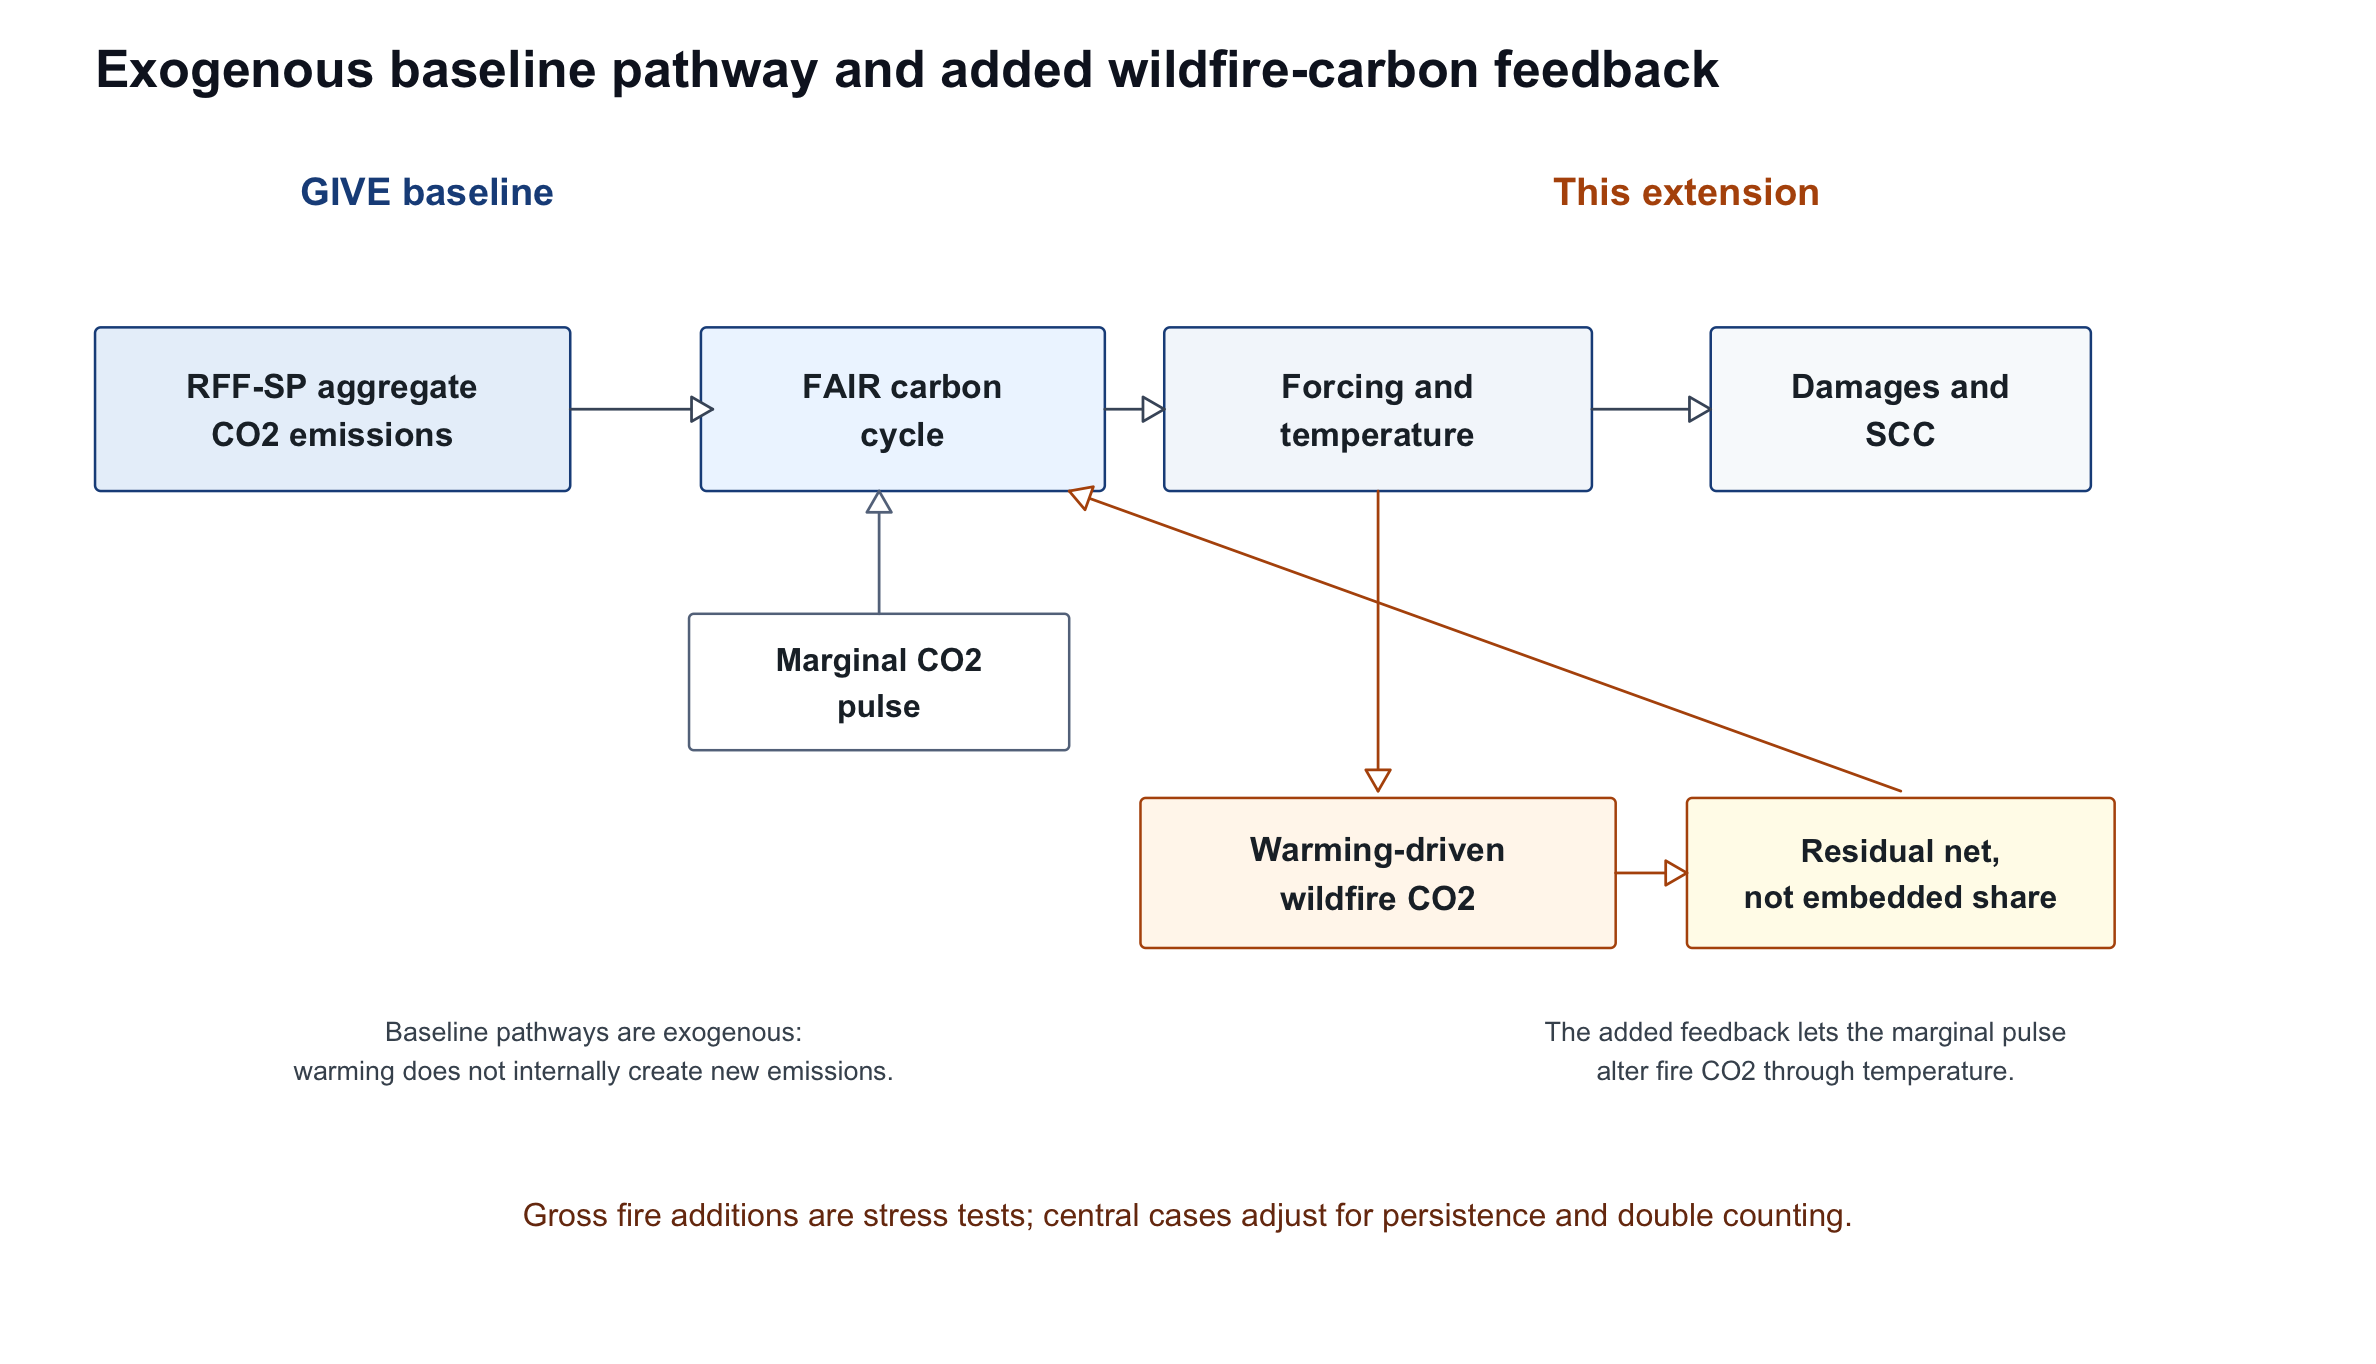
\includegraphics[width=0.78\linewidth,height=\textheight,keepaspectratio,alt={Exogenous baseline pathway and added wildfire-carbon feedback. GIVE carries aggregate CO2 emissions through the carbon cycle, forcing, temperature and damages. The extension adds a temperature-dependent fire-carbon pathway before the carbon cycle and scales it by persistence and accounting uncertainty.}]{figures/png_pdf/figure_conceptual_audit_schematic.png}
\caption{Exogenous baseline pathway and added wildfire-carbon feedback.
GIVE carries aggregate CO2 emissions through the carbon cycle, forcing,
temperature and damages. The extension adds a temperature-dependent
fire-carbon pathway before the carbon cycle and scales it by persistence
and accounting uncertainty.}
\end{figure}

\subsubsection{A residual feedback limits double
counting}\label{a-residual-feedback-limits-double-counting}

We model added fire CO2 as a reduced-form response to lagged global mean
temperature above the 2020 reference level. Annual added fire emissions
equal a reference gross fire-carbon flux multiplied by a
temperature-response slope, a net-persistence fraction and a
not-already-embedded fraction. These three terms separate different
uncertainties. The gross temperature response is a physical fire-model
uncertainty. The net-persistence fraction is a carbon-cycle uncertainty:
regrowth, changing future sink strength, pyrogenic carbon and soil
carbon determine whether gross combustion becomes durable atmospheric
CO2. The not-already-embedded fraction is an accounting uncertainty, not
a physical parameter. It represents the share of the feedback not
already captured in RFF-SP aggregate CO2.

The residual-medium scenario is deliberately conservative. It assumes a
modest temperature response, low net persistence and partial embedding
in baseline emissions. The residual-high scenario allows a stronger
climate-fire response and a larger missing share, but still treats gross
fire emissions as only partly persistent and only partly absent from the
baseline. The RESFire-style stress cases remove these protections by
setting persistence and missing fractions to one and calibrating the
response to high forest-fire projections. They are useful for testing
the mechanism; they are not double-counting-safe central estimates.

We make the source-side accounting assumption explicit with a
qualitative global proxy. The proxy is not an observed emissions
inventory, not a GIVE model output and not a damage map. It is a
transparent 0-1 index for regions where climate-sensitive fire-carbon
additions are most plausible in the literature, with a residual version
that downweights places where gross fire emissions are more likely to
overlap with AFOLU inventories, managed burning, rapid regrowth or
aggregate-emissions expectations. The point is not to allocate welfare
impacts by country; it is to make the assumed source of the added carbon
visible.

\begin{figure}
\centering
\pandocbounded{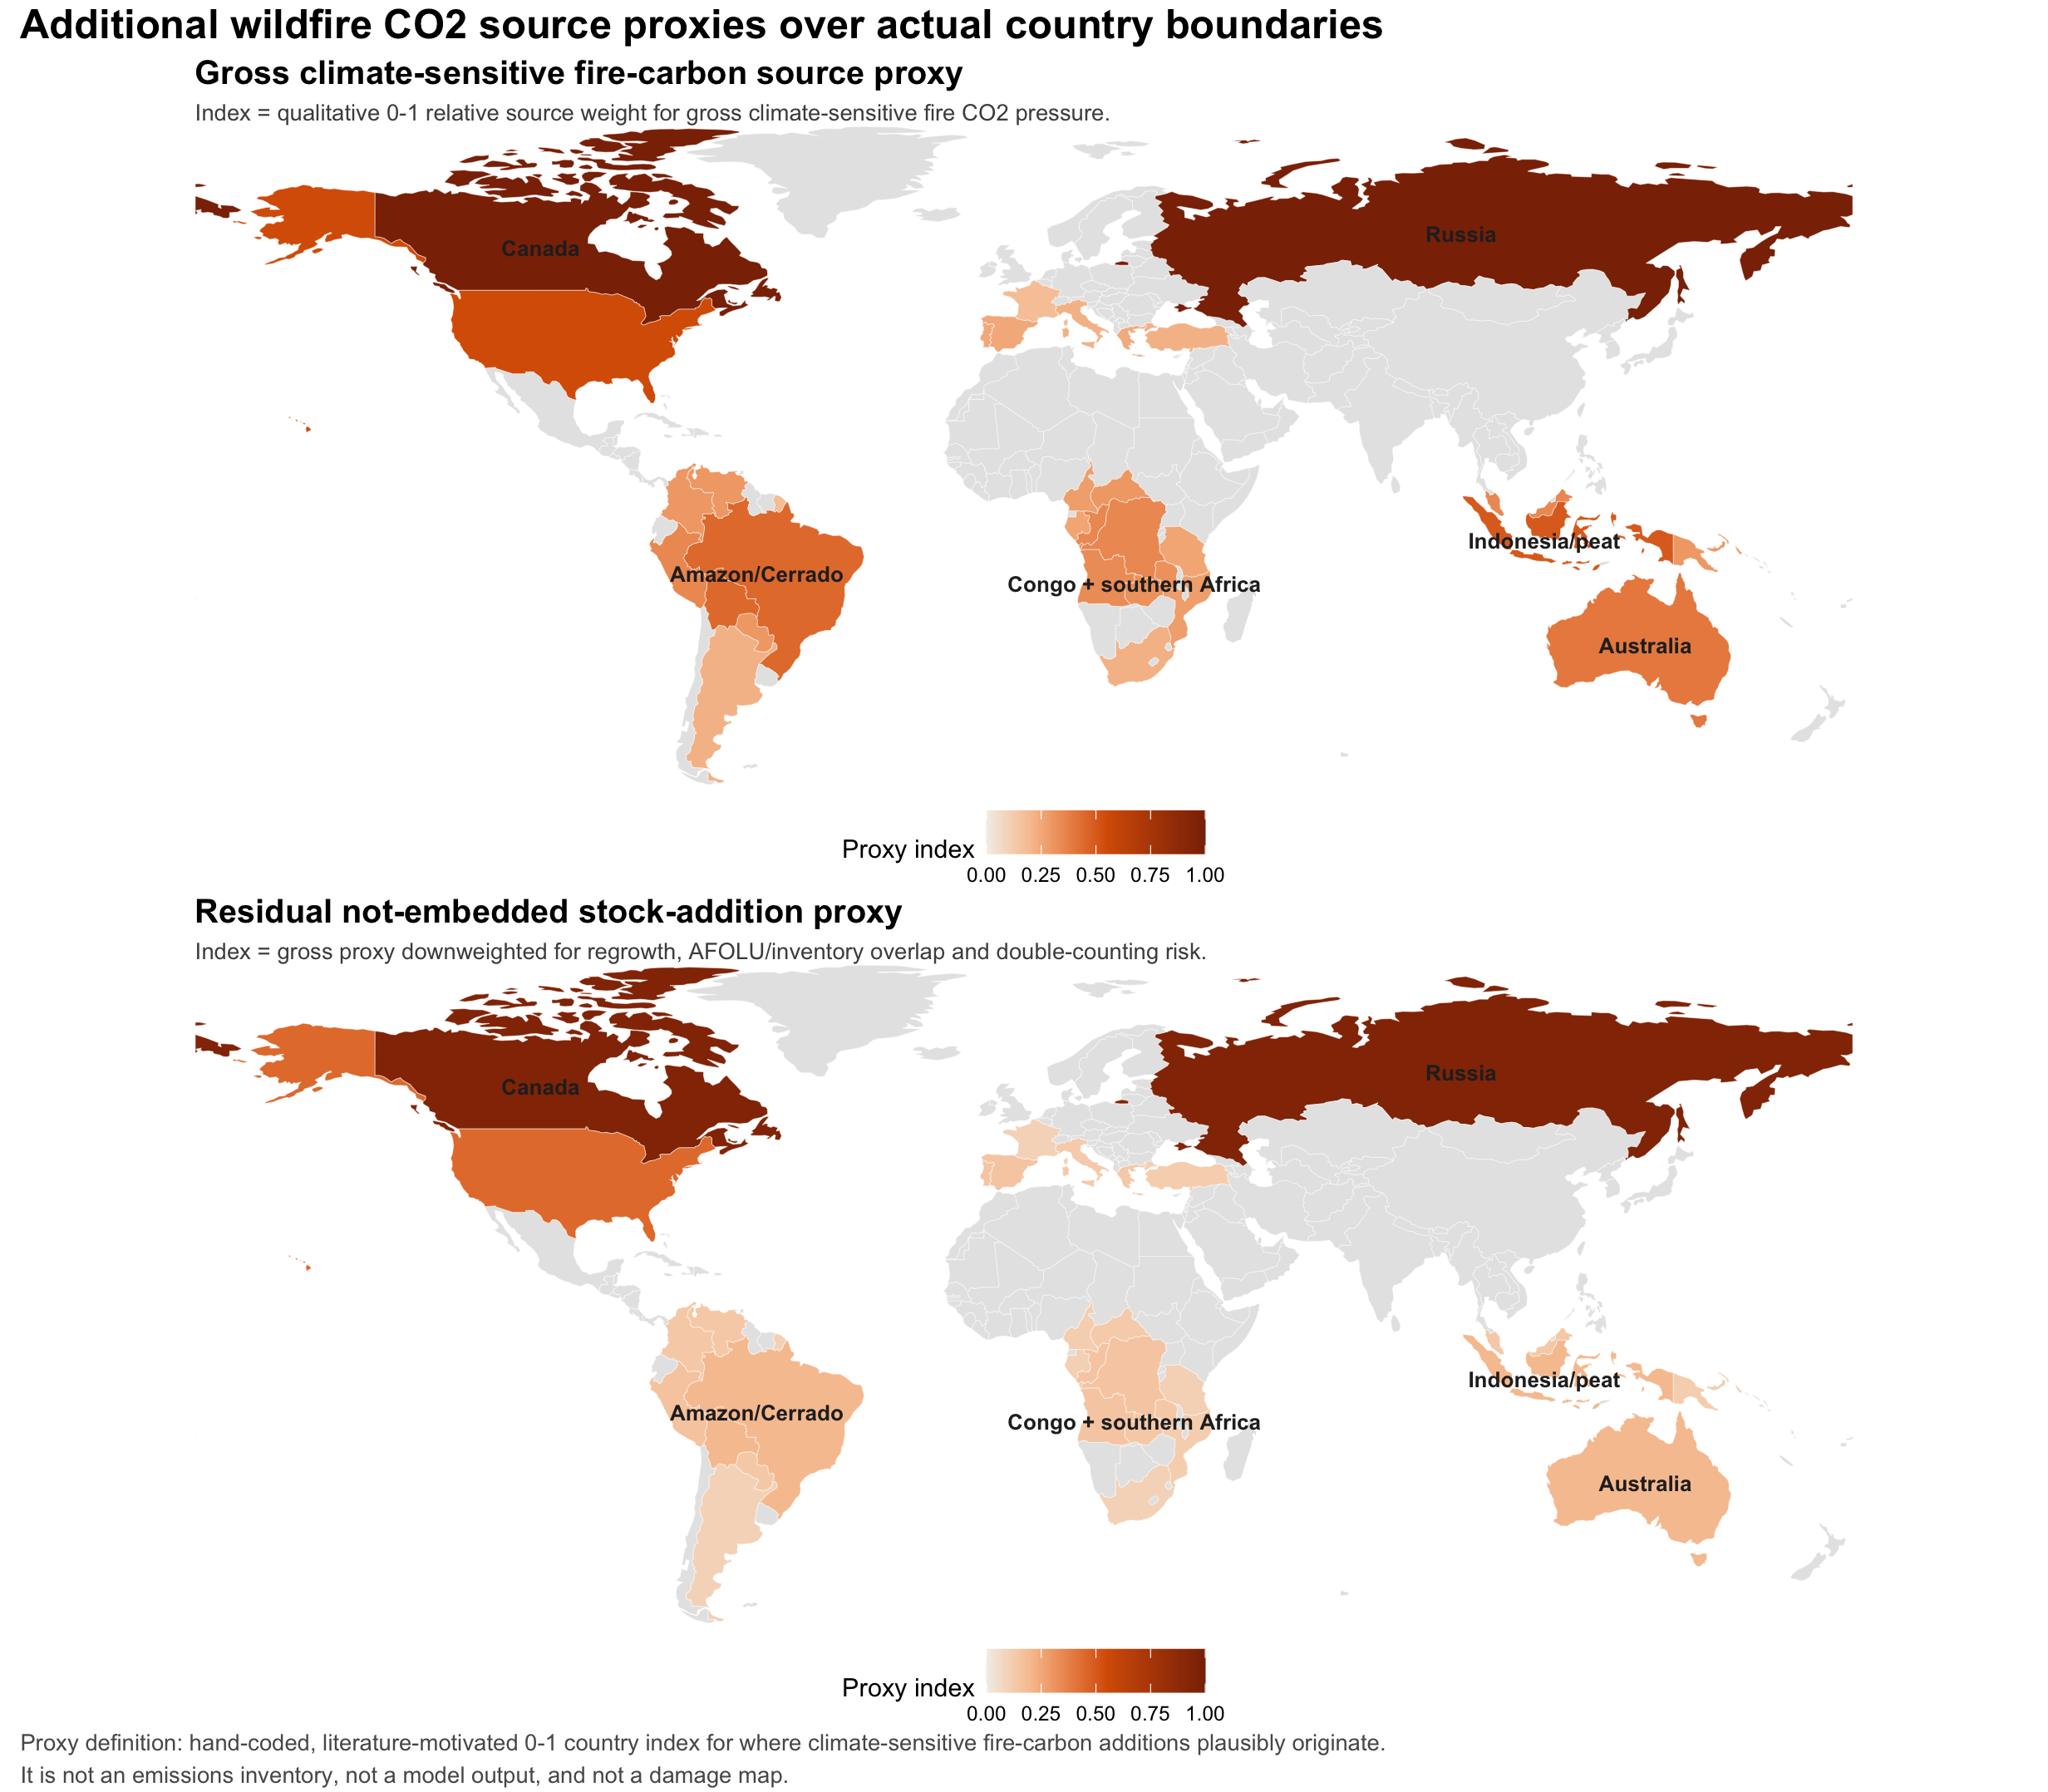
\includegraphics[keepaspectratio,alt={Source-side proxy for additional wildfire CO2. The gross source index highlights broad climate-sensitive fire-carbon regions, while the residual index downweights areas with higher risk of double counting through AFOLU, managed burning, regrowth or baseline aggregate-emissions expectations.}]{figures/png_pdf/figure_fire_source_country_proxy_map.png}}
\caption{Source-side proxy for additional wildfire CO2. The gross source
index highlights broad climate-sensitive fire-carbon regions, while the
residual index downweights areas with higher risk of double counting
through AFOLU, managed burning, regrowth or baseline aggregate-emissions
expectations.}
\end{figure}

\subsubsection{Fire-carbon scale depends on flow versus
stock}\label{fire-carbon-scale-depends-on-flow-versus-stock}

The fire-carbon pathway is more visible as an annual flow than as an
atmospheric stock increment. In the source-informed mean pathway used
for diagnostics, added wildfire CO2 is 1.03 GtCO2/yr in 2050 and 1.23
GtCO2/yr in 2100. These amounts equal 2.34\% and 4.50\% of GIVE's
baseline annual aggregate CO2 emissions in those years. The
corresponding atmospheric CO2-C stock additions are 0.28\% in 2050 and
1.05\% in 2100. The difference between these percentages explains why a
Canada-2023-scale fire year can be large relative to annual emissions
but small relative to total atmospheric carbon.

The residual scenarios are smaller. Residual-medium adds 0.024 GtCO2/yr
in 2050 and 0.056 GtCO2/yr in 2100, with atmospheric-stock additions
below 0.04\% by 2100. Residual-high reaches 1.27 GtCO2/yr by 2100, equal
to 4.63\% of baseline annual CO2 emissions and 0.80\% of the atmospheric
CO2-C stock. The gross stress case is much larger: 7.80 GtCO2/yr in 2050
and 20.54 GtCO2/yr in 2100, equal to 17.63\% and 75.11\% of baseline
annual emissions, with atmospheric-stock increases of 2.01\% and
12.37\%. These values are useful scale tests but should not be
interpreted as preferred fire-carbon projections.

\begin{figure}
\centering
\pandocbounded{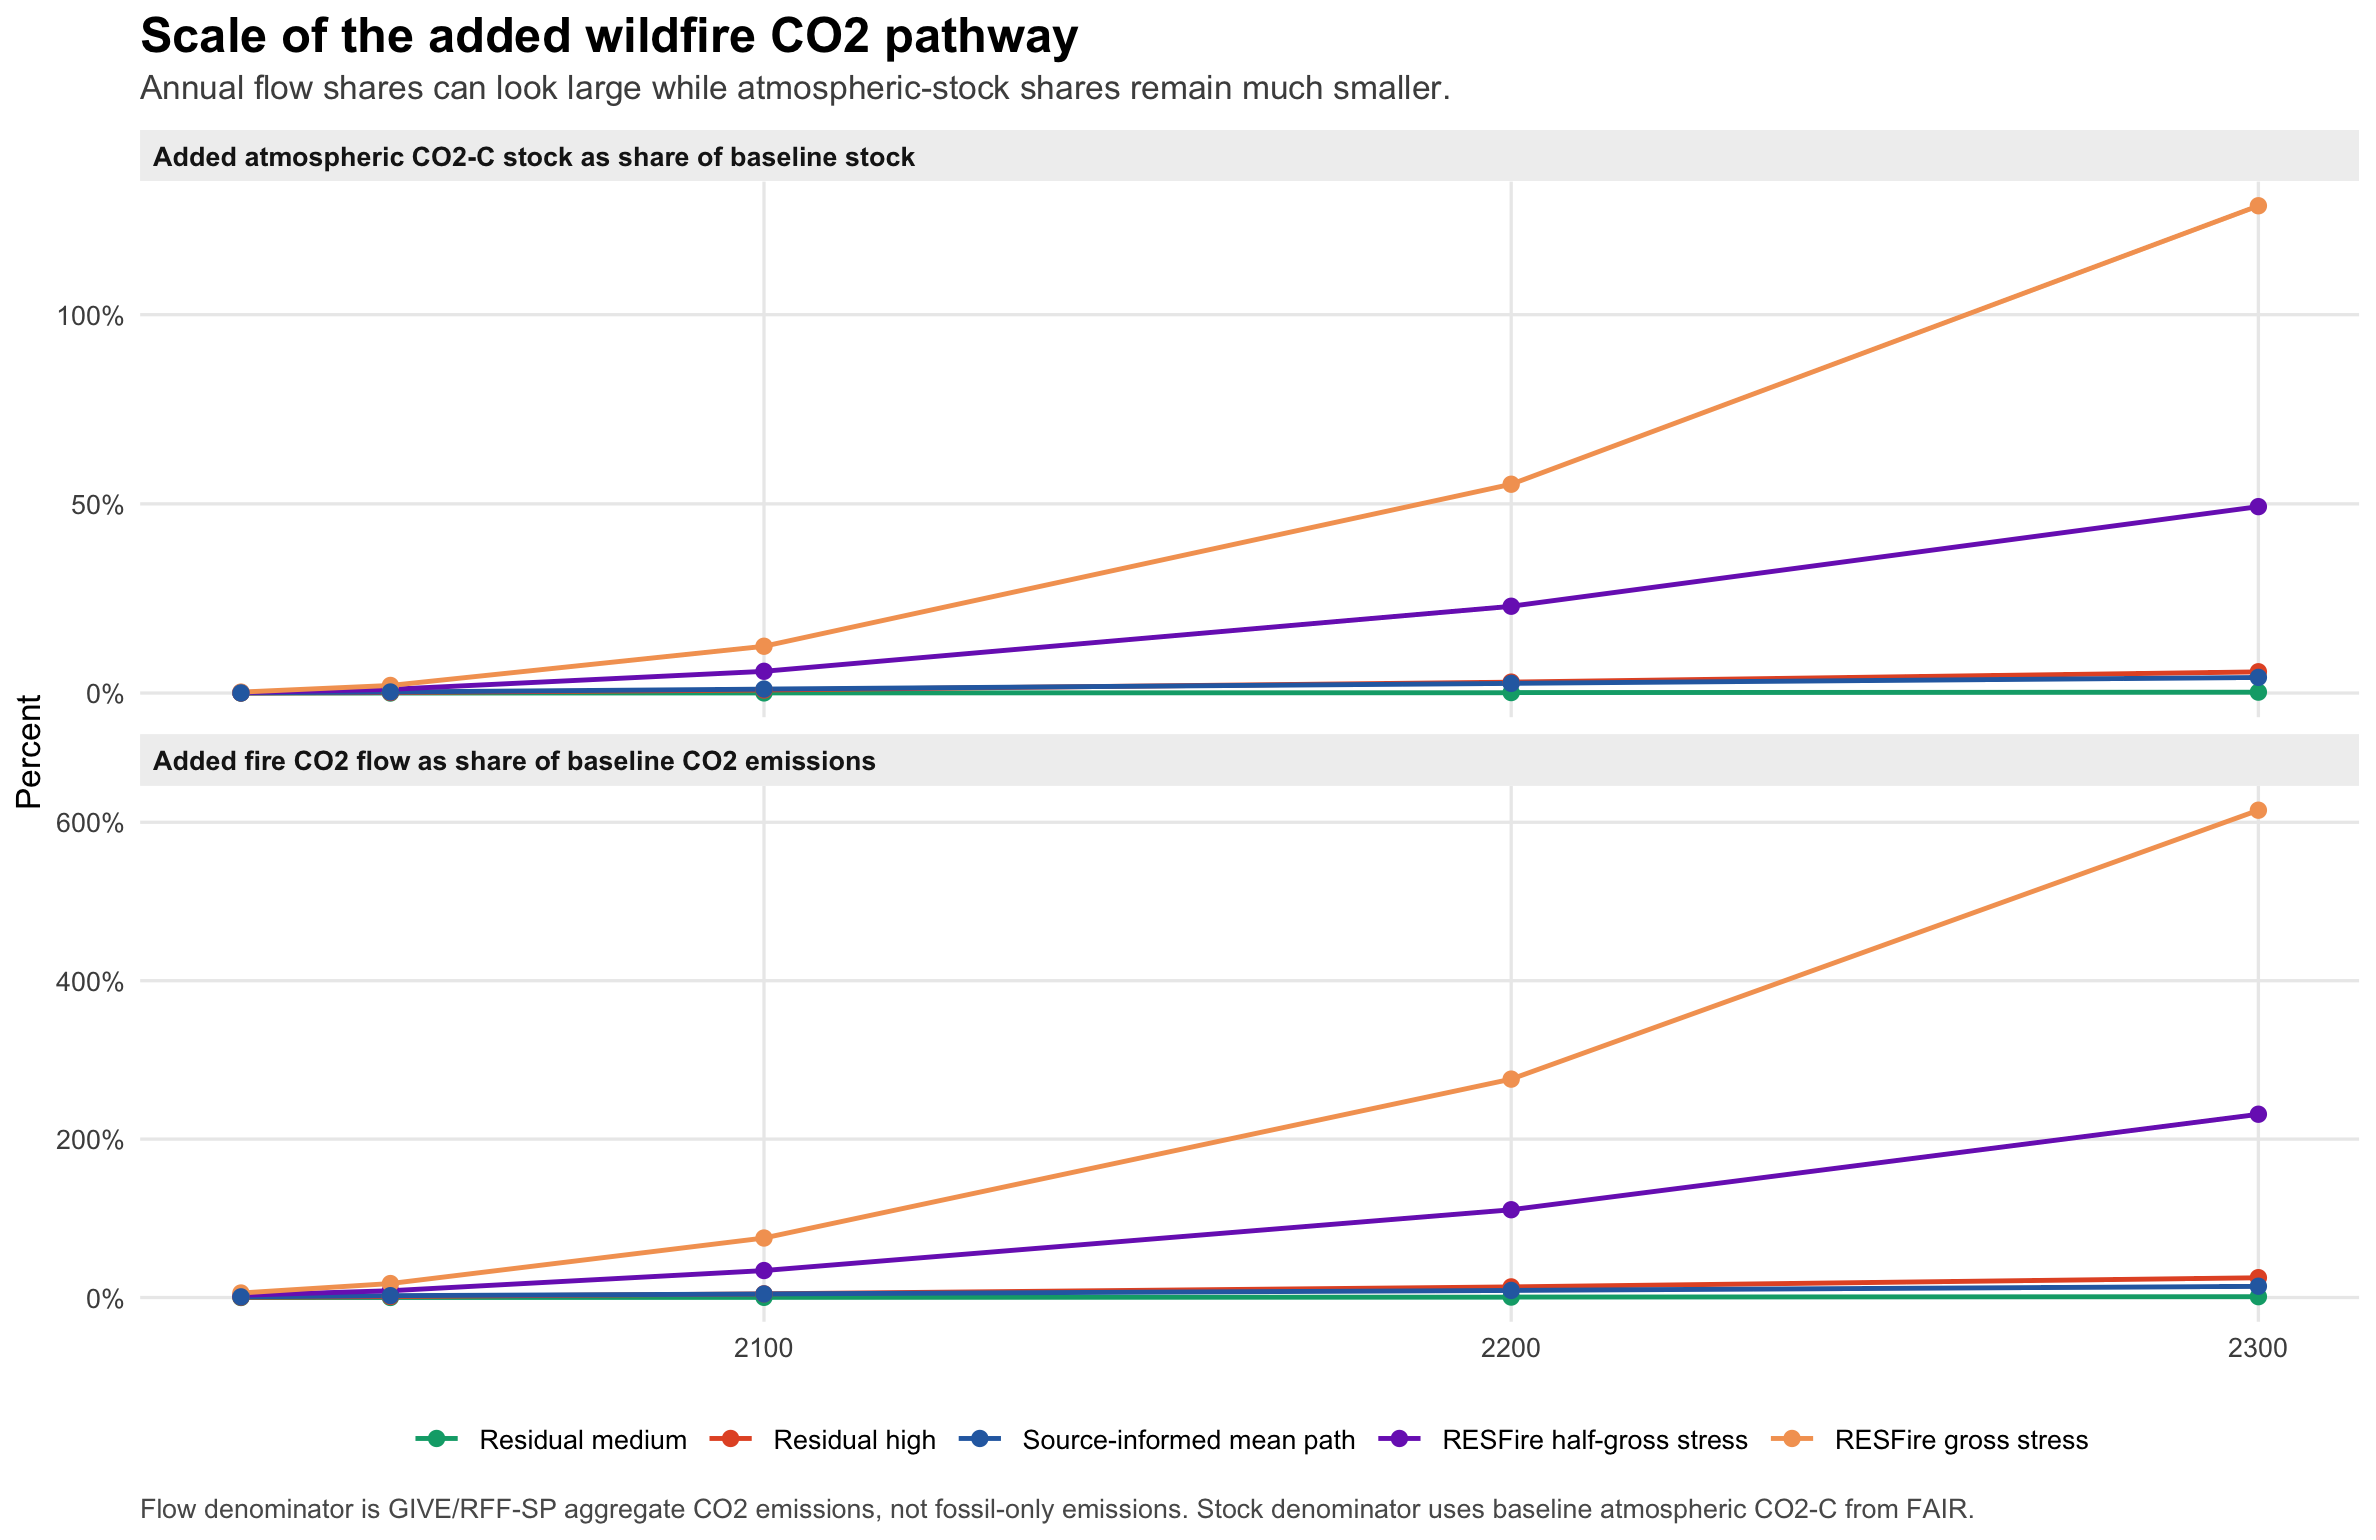
\includegraphics[keepaspectratio,alt={Fire-carbon accounting scale. Annual added wildfire CO2 can be several percent of baseline annual emissions while remaining much smaller as a percentage of the atmospheric carbon stock.}]{figures/png_pdf/figure_fire_scale_shares.png}}
\caption{Fire-carbon accounting scale. Annual added wildfire CO2 can be
several percent of baseline annual emissions while remaining much
smaller as a percentage of the atmospheric carbon stock.}
\end{figure}

\subsubsection{Residual feedbacks modestly raise SCC in validation
runs}\label{residual-feedbacks-modestly-raise-scc-in-validation-runs}

In the deterministic 2.0\% discount case, the baseline SCC is 139.10
2020 USD/tCO2. Residual-medium increases it by 0.15 USD/tCO2 (+0.11\%).
Residual-high increases it by 5.60 USD/tCO2 (+4.02\%). The half-gross
and gross stress cases increase it by 39.30 and 78.76 USD/tCO2,
respectively. The deterministic model therefore confirms that the
feedback is wired into the carbon cycle and damages, and that the
response is strongly scenario-dependent.

We then implemented a paired Monte Carlo design that holds the same
socioeconomic, climate, damage and discounting draws across baseline and
wildfire scenarios. Pairing reduces sampling noise in scenario
differences. In the corrected 100-draw validation run, the baseline
2.0\% SCC mean is 198.35 2020 USD/tCO2 and the median is 155.82 2020
USD/tCO2. This is close to Rennert et al.'s preferred mean given the
small sample and the right-skewed SCC distribution. A larger production
driver is configured, but the current draft reports 100-draw validation
values and should be interpreted as a model-development result.

Residual-medium raises the 100-draw mean by 0.54 USD/tCO2 (+0.27\%).
Residual-high raises it by 11.21 USD/tCO2 (+5.65\%). The half-gross
stress case raises it by 64.44 USD/tCO2 (+32.49\%), and the gross stress
case by 148.02 USD/tCO2 (+74.62\%). The right tail is large, so Figure 4
truncates the displayed density at 600 USD/tCO2 while computing means
and medians on the full sample. The paired-delta panel shows that the
gross stress cases shift nearly all draws upward, whereas residual cases
are much smaller and more sensitive to draw-level model states.

\begin{figure}
\centering
\pandocbounded{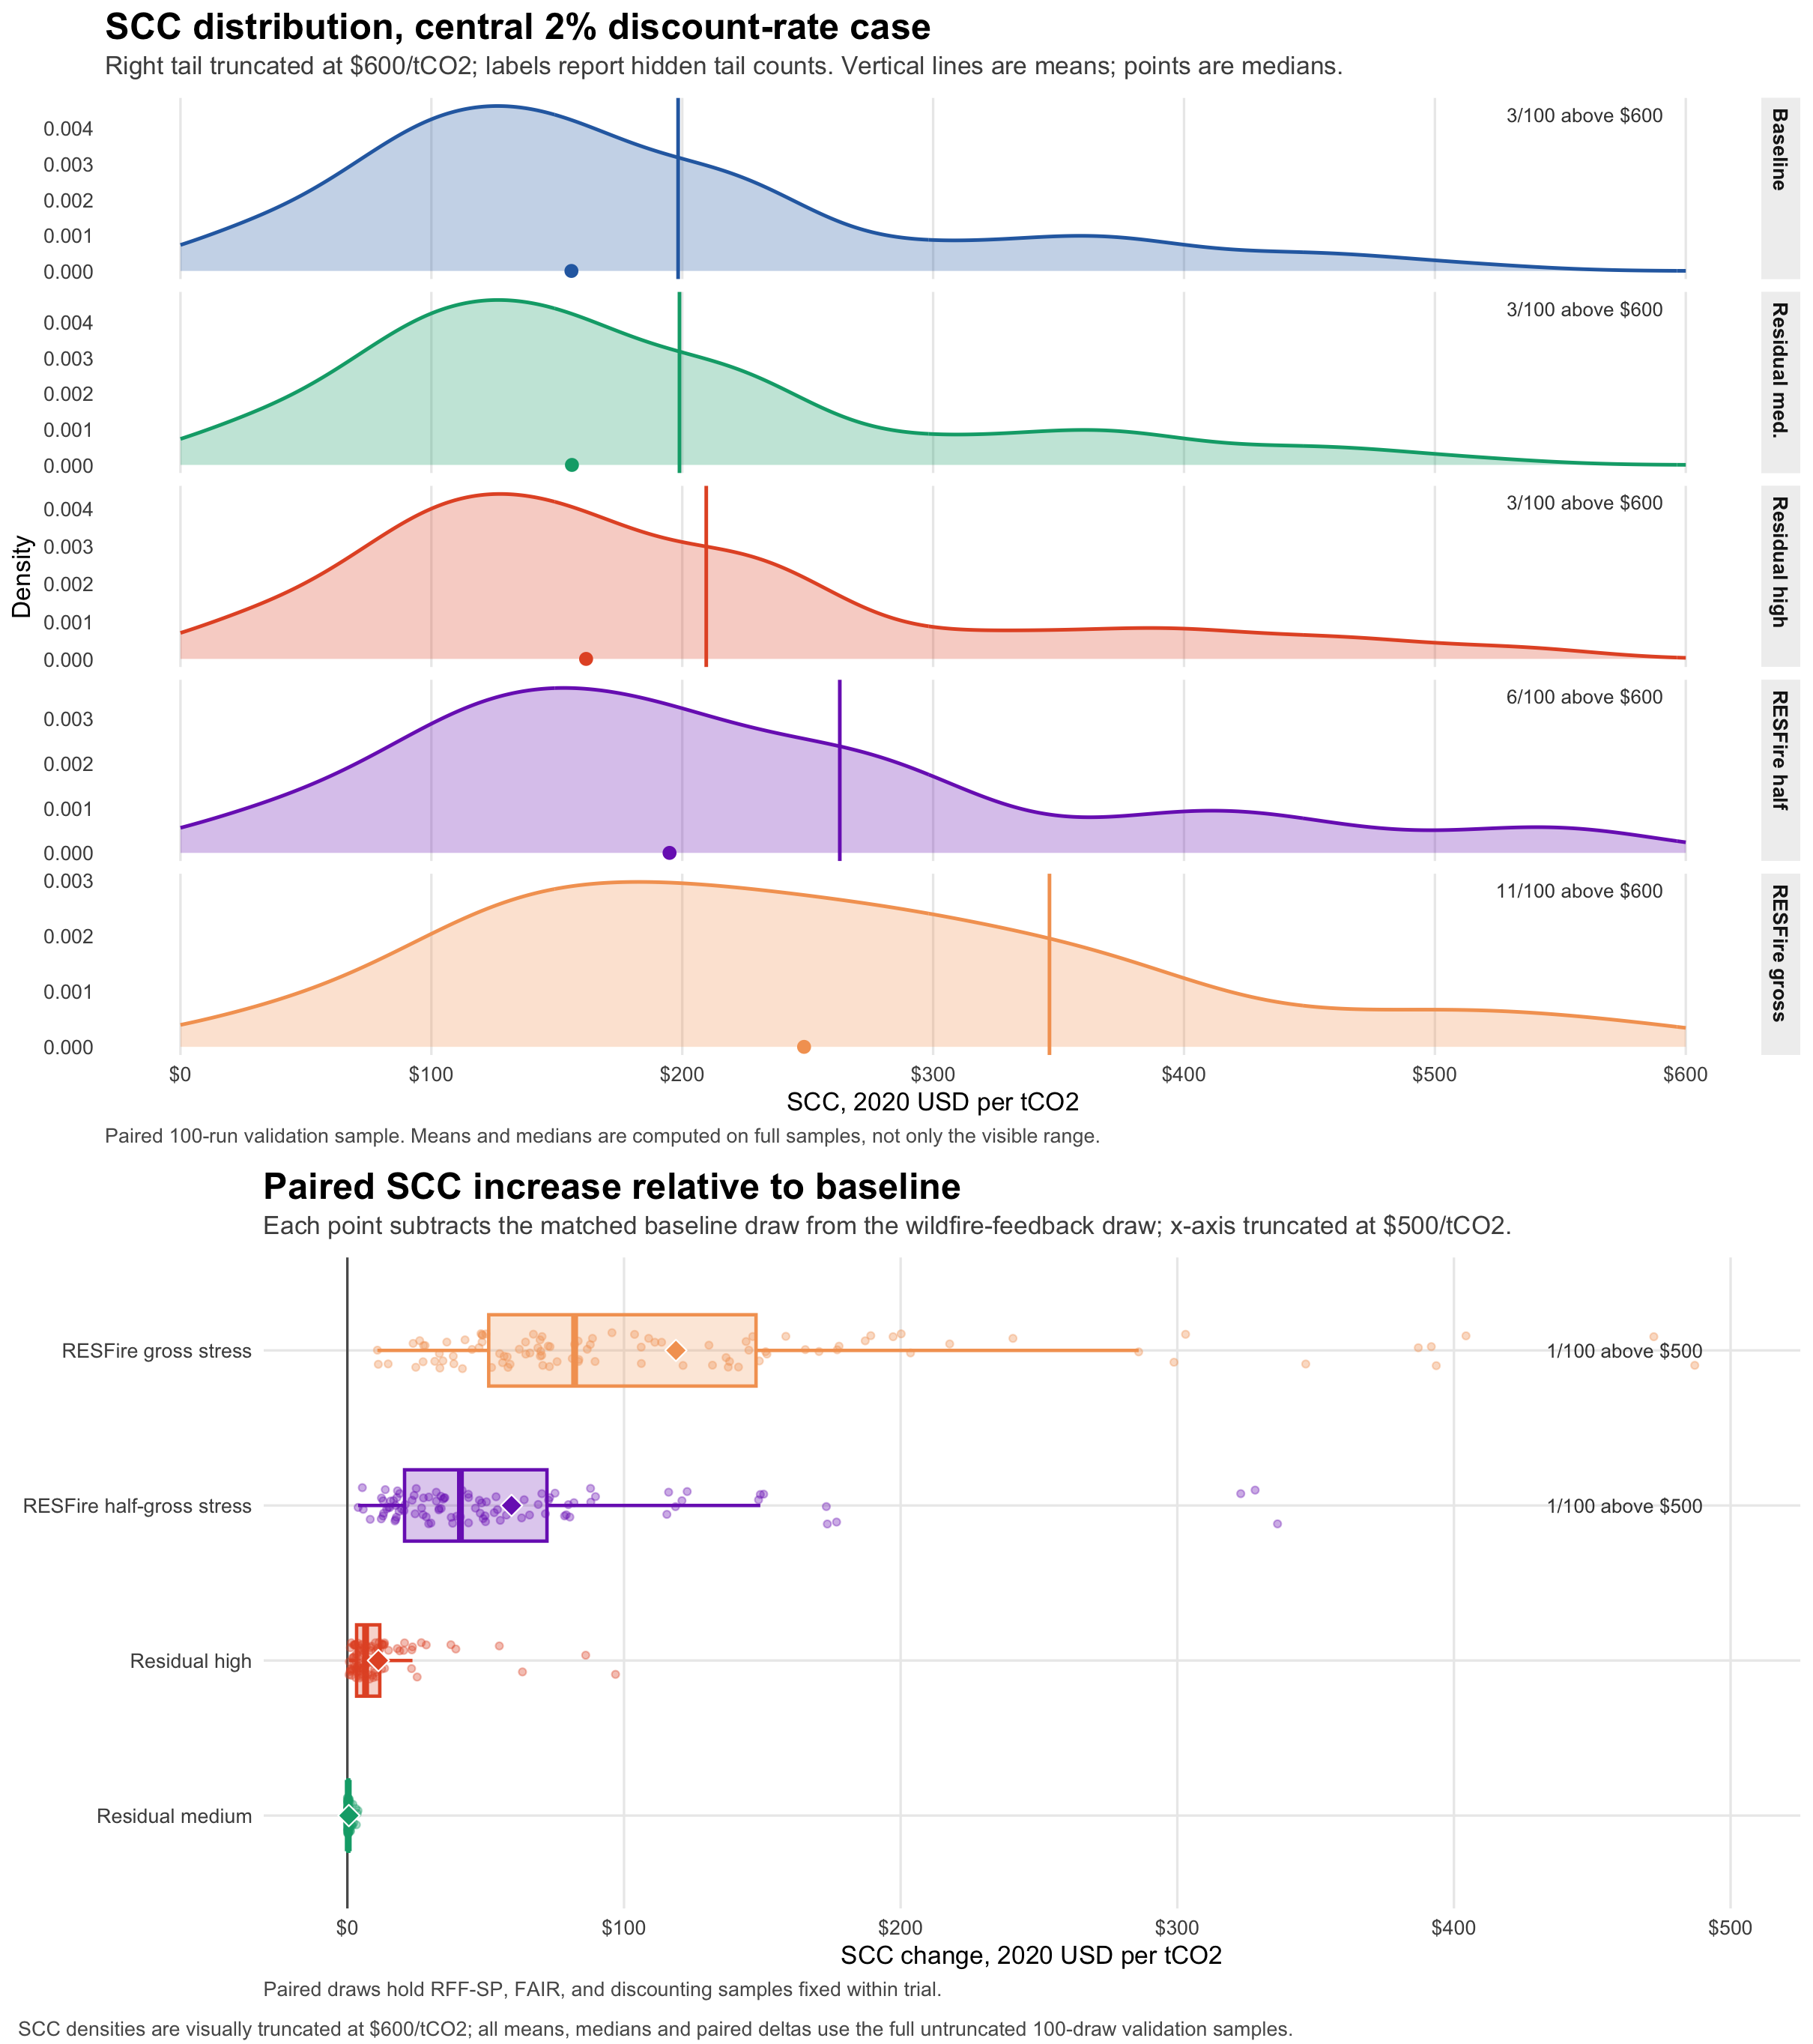
\includegraphics[keepaspectratio,alt={SCC distributions and paired scenario deltas. Densities are truncated visually at 600 USD/tCO2; means, medians and paired deltas are computed on the untruncated samples. Each point in the lower panel subtracts the matched baseline draw from the wildfire-feedback draw.}]{figures/png_pdf/figure_scc_distribution_and_delta_2pct.png}}
\caption{SCC distributions and paired scenario deltas. Densities are
truncated visually at 600 USD/tCO2; means, medians and paired deltas are
computed on the untruncated samples. Each point in the lower panel
subtracts the matched baseline draw from the wildfire-feedback draw.}
\end{figure}

{\def\LTcaptype{none} % do not increment counter
\begin{longtable}[]{@{}
  >{\raggedright\arraybackslash}p{(\linewidth - 12\tabcolsep) * \real{0.1111}}
  >{\raggedleft\arraybackslash}p{(\linewidth - 12\tabcolsep) * \real{0.1481}}
  >{\raggedleft\arraybackslash}p{(\linewidth - 12\tabcolsep) * \real{0.1481}}
  >{\raggedleft\arraybackslash}p{(\linewidth - 12\tabcolsep) * \real{0.1481}}
  >{\raggedleft\arraybackslash}p{(\linewidth - 12\tabcolsep) * \real{0.1481}}
  >{\raggedleft\arraybackslash}p{(\linewidth - 12\tabcolsep) * \real{0.1481}}
  >{\raggedleft\arraybackslash}p{(\linewidth - 12\tabcolsep) * \real{0.1481}}@{}}
\toprule\noalign{}
\begin{minipage}[b]{\linewidth}\raggedright
Scenario
\end{minipage} & \begin{minipage}[b]{\linewidth}\raggedleft
Mean SCC
\end{minipage} & \begin{minipage}[b]{\linewidth}\raggedleft
Median SCC
\end{minipage} & \begin{minipage}[b]{\linewidth}\raggedleft
5th
\end{minipage} & \begin{minipage}[b]{\linewidth}\raggedleft
95th
\end{minipage} & \begin{minipage}[b]{\linewidth}\raggedleft
Delta mean
\end{minipage} & \begin{minipage}[b]{\linewidth}\raggedleft
Delta \%
\end{minipage} \\
\midrule\noalign{}
\endhead
\bottomrule\noalign{}
\endlastfoot
Baseline & 198.35 & 155.82 & 33.39 & 464.21 & 0.00 & 0.00\% \\
Residual medium & 198.89 & 156.03 & 33.46 & 465.23 & 0.54 & 0.27\% \\
Residual high & 209.57 & 161.67 & 35.80 & 485.26 & 11.21 & 5.65\% \\
RESFire half-gross stress & 262.79 & 194.93 & 45.45 & 646.43 & 64.44 &
32.49\% \\
RESFire gross stress & 346.37 & 248.55 & 84.63 & 785.47 & 148.02 &
74.62\% \\
\end{longtable}
}

Paired-delta intervals are more informative than SCC-level intervals for
this question. In the validation sample, residual-medium has a 5-95\%
paired-delta interval of 0.06-2.00 USD/tCO2 and never exceeds 10
USD/tCO2. Residual-high has a 5-95\% interval of 1.25-37.51 USD/tCO2,
and 34\% of paired draws exceed 10 USD/tCO2. The half-gross and gross
stress cases have 5-95\% intervals of 12.32-173.66 and 26.08-391.90
USD/tCO2. The probability of a positive delta is 100\% in this 100-draw
validation sample for all four feedback cases; this should be read as a
paired-sample diagnostic, not as a final posterior probability.

\begin{figure}
\centering
\pandocbounded{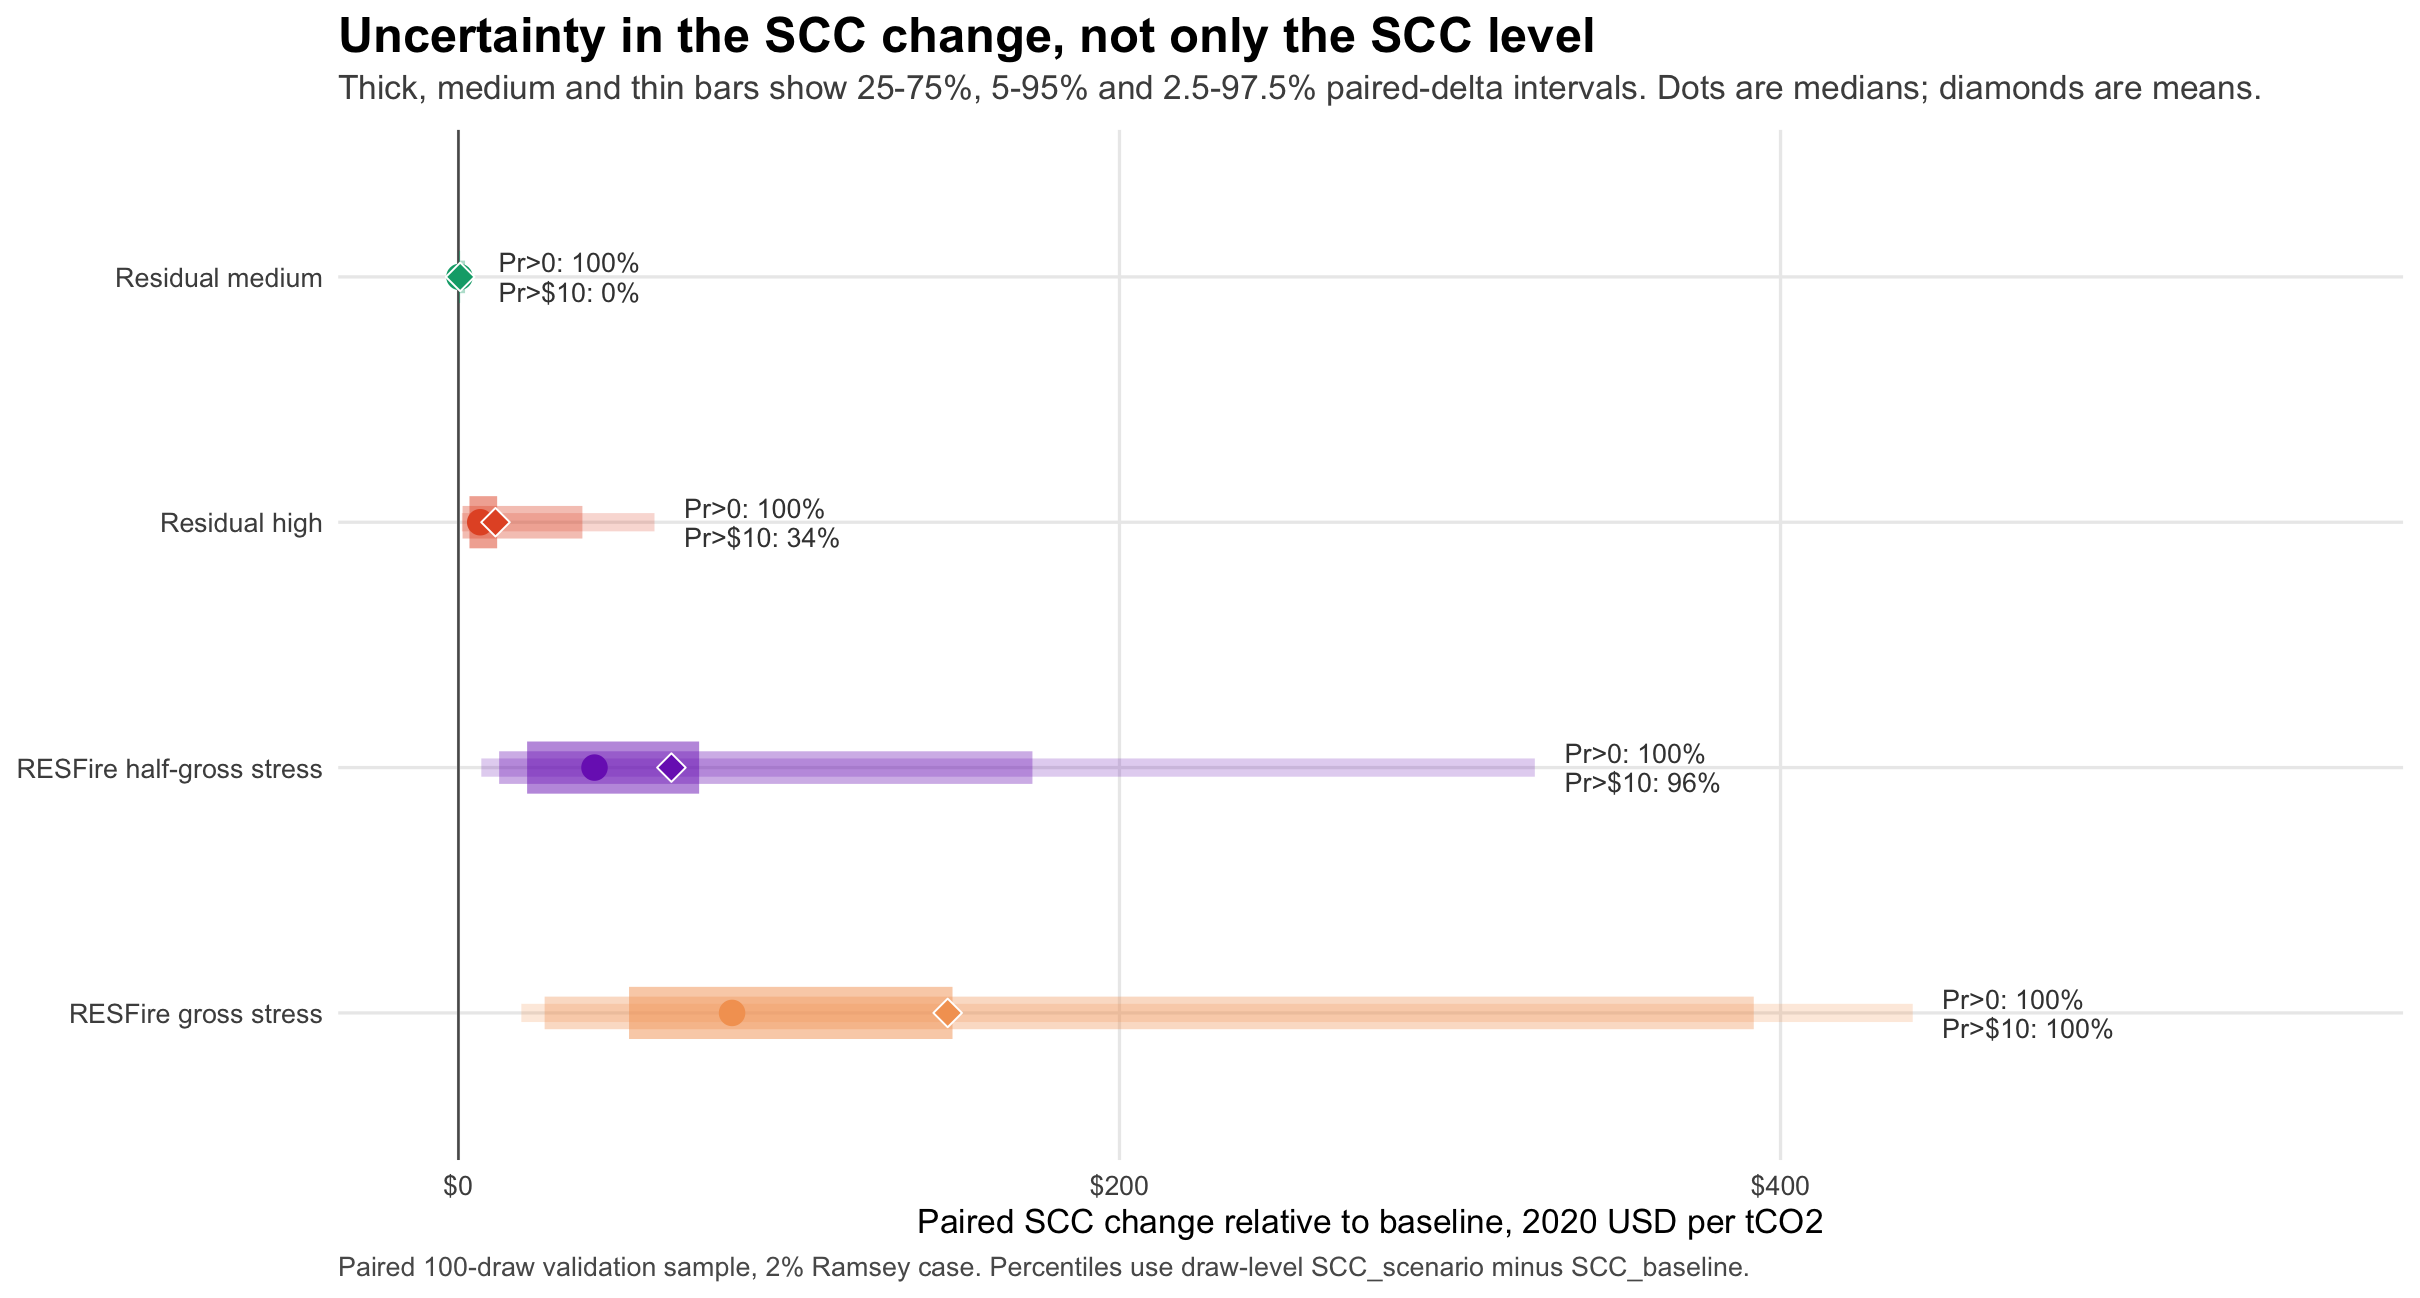
\includegraphics[keepaspectratio,alt={Paired-delta uncertainty intervals. Thick, medium and thin bars show 25-75\%, 5-95\% and 2.5-97.5\% paired-delta intervals for the 2\% case. Dots are medians and diamonds are means.}]{figures/png_pdf/figure_paired_delta_intervals_2pct.png}}
\caption{Paired-delta uncertainty intervals. Thick, medium and thin bars
show 25-75\%, 5-95\% and 2.5-97.5\% paired-delta intervals for the 2\%
case. Dots are medians and diamonds are means.}
\end{figure}

\subsubsection{Accounting uncertainty dominates
interpretation}\label{accounting-uncertainty-dominates-interpretation}

The uncertainty structure matters as much as the point estimate. The
residual scenarios sample over physical response, net persistence and
missing-share terms. The stress scenarios instead set net persistence
and missing share to one. That makes them useful for mechanism
detection, but it also removes the two protections against double
counting. The parameter draws are therefore best interpreted as bounded
accounting scenarios rather than as a formal posterior distribution over
global fire-carbon feedbacks.

The 100-draw design also clarifies what the current experiment can and
cannot separate. Baseline GIVE uncertainty is large: the 2\% baseline
SCC has a standard deviation of 156.02 USD/tCO2 in the validation
sample. The residual-medium paired-delta standard deviation is only 0.72
USD/tCO2, and the residual-high paired-delta standard deviation is 15.54
USD/tCO2. Simple proxy regressions suggest that both baseline model
state and effective feedback intensity help explain residual-case delta
variation. For residual-high, the baseline SCC draw alone explains 51\%
of paired-delta variation, the effective fire-feedback intensity
explains 26\%, and both together explain 68\%. This diagnostic is not a
formal variance decomposition because GIVE and wildfire-parameter draws
are paired rather than factorially crossed. It does, however, show that
final uncertainty quantification should report both baseline SCC
uncertainty and uncertainty in the added fire-carbon accounting terms.

\begin{figure}
\centering
\pandocbounded{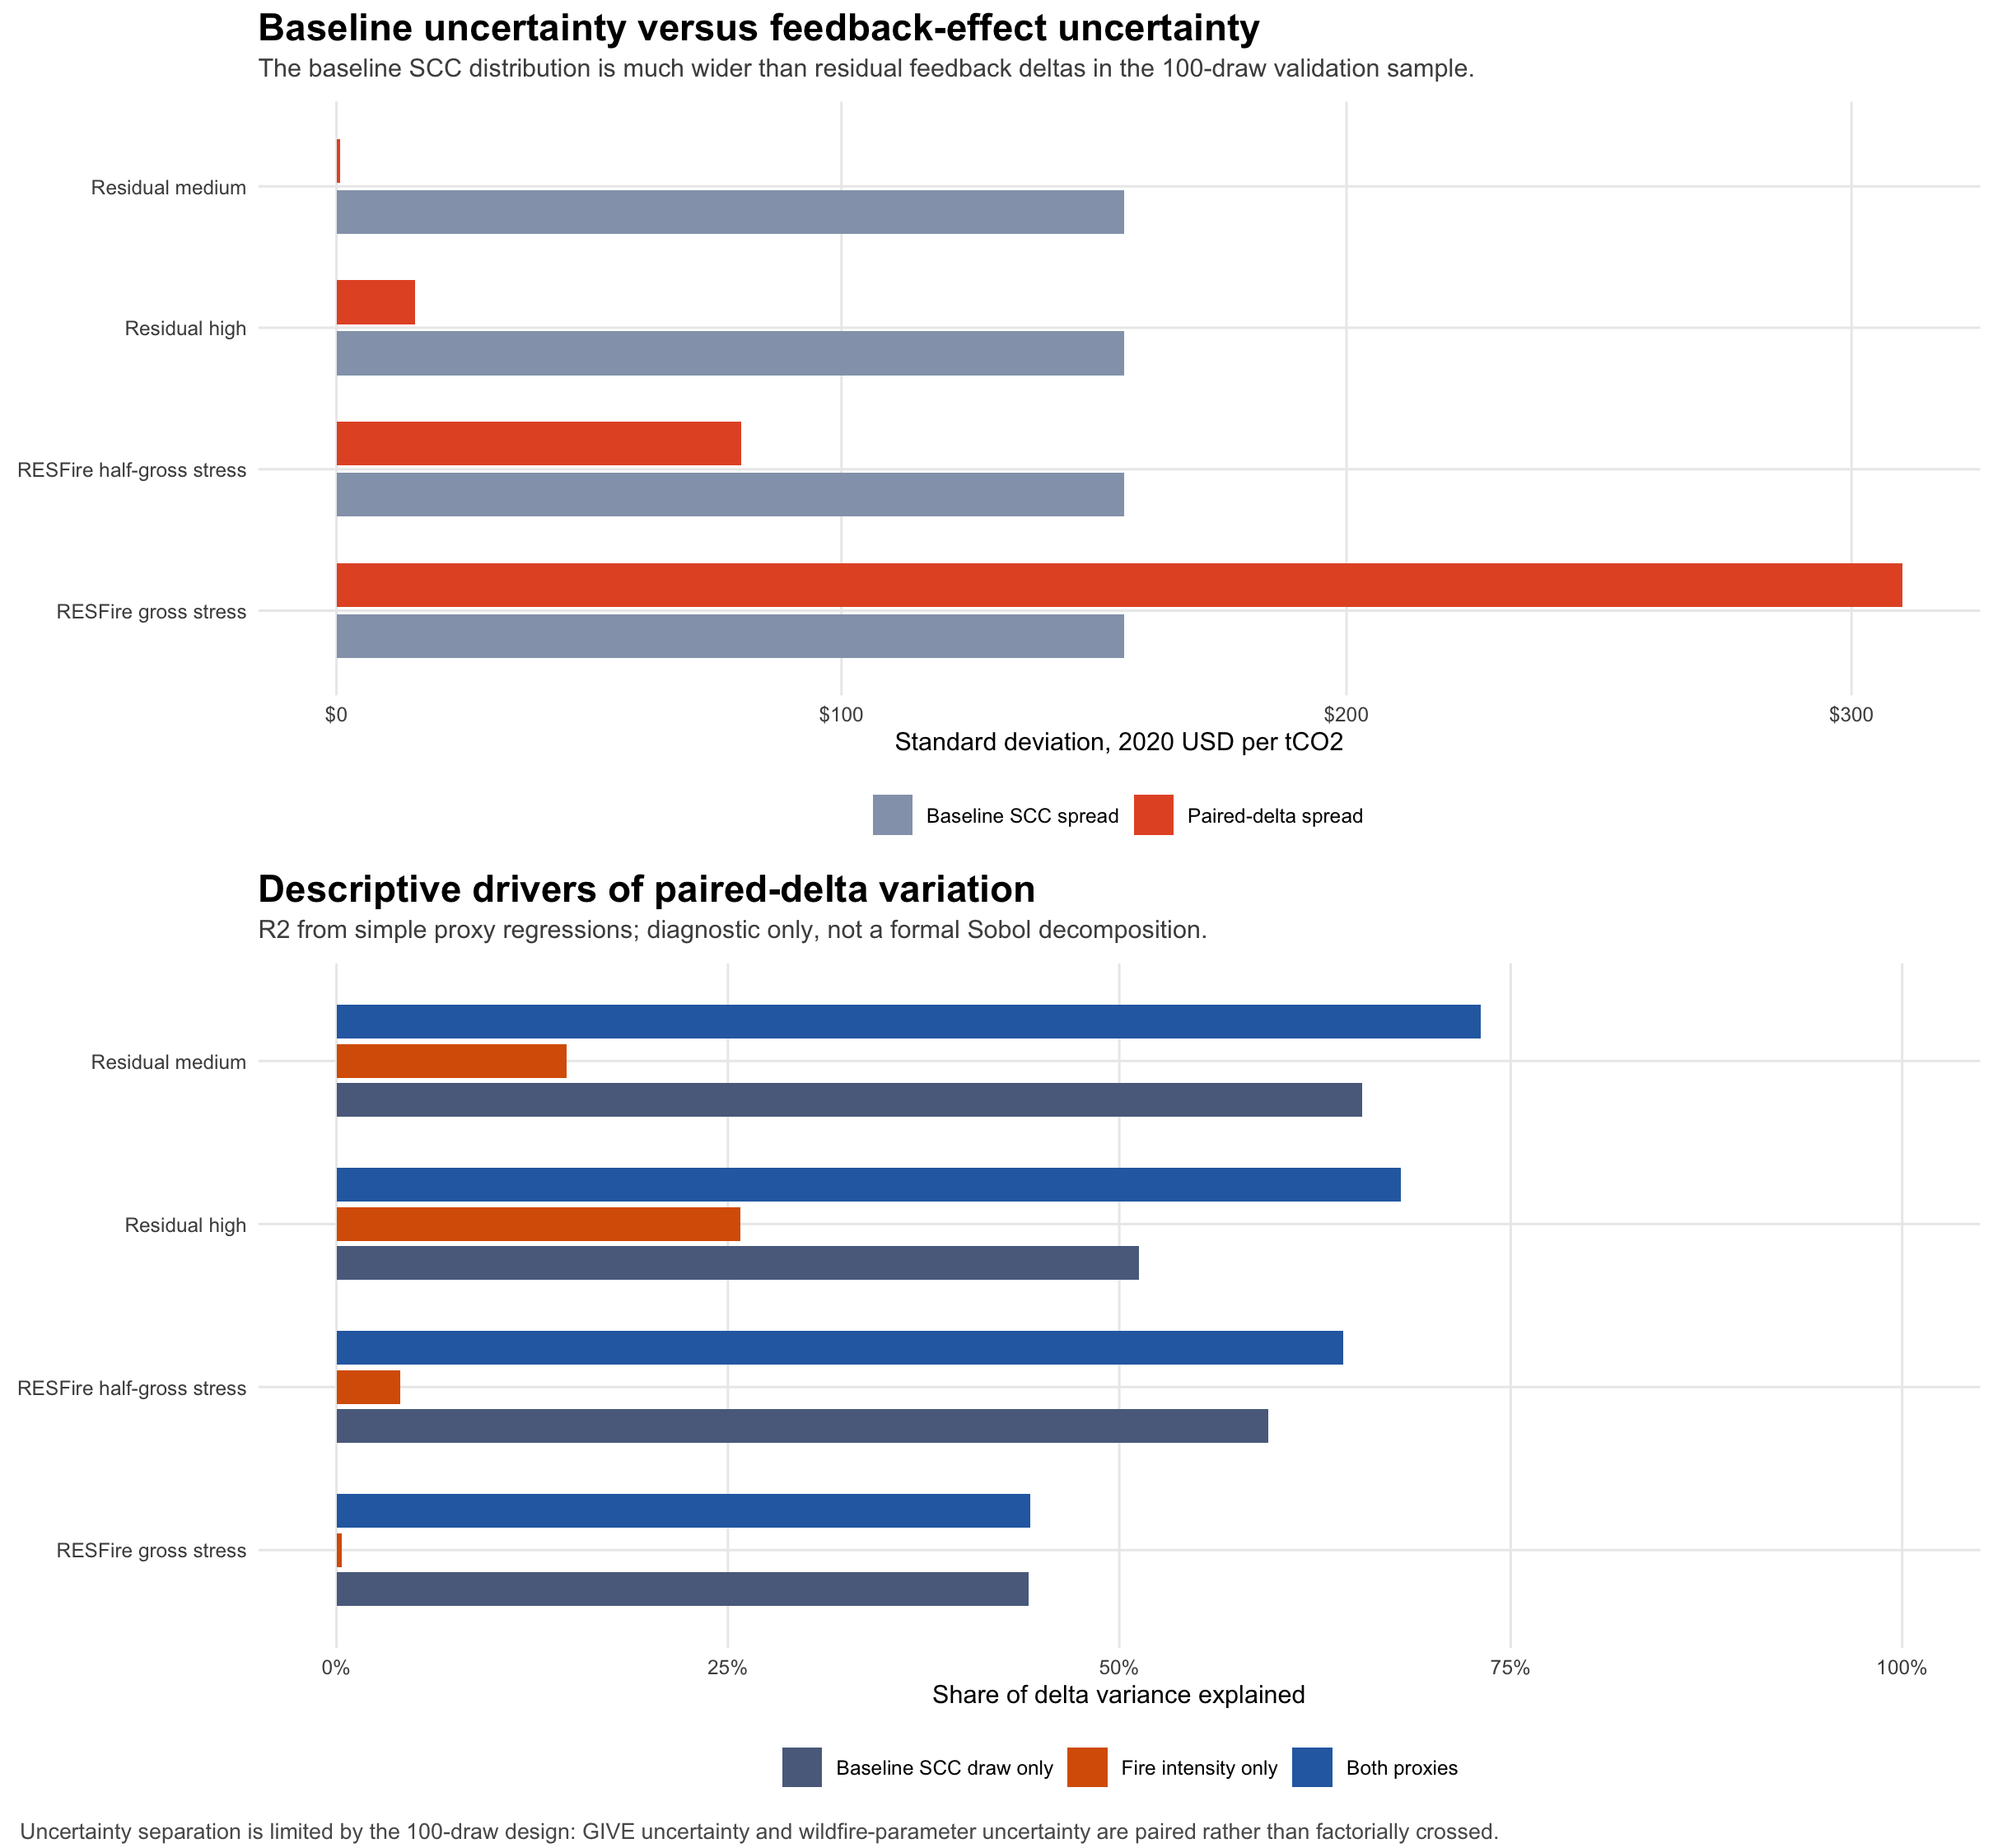
\includegraphics[keepaspectratio,alt={Uncertainty-source diagnostics. The top panel compares the spread of baseline SCC draws with the spread of paired wildfire-feedback deltas. The lower panel reports simple proxy-regression R2 values for baseline SCC state, effective fire-feedback intensity and both proxies.}]{figures/png_pdf/figure_uncertainty_source_diagnostics_2pct.png}}
\caption{Uncertainty-source diagnostics. The top panel compares the
spread of baseline SCC draws with the spread of paired wildfire-feedback
deltas. The lower panel reports simple proxy-regression R2 values for
baseline SCC state, effective fire-feedback intensity and both proxies.}
\end{figure}

\subsubsection{Mechanisms are muted by marginal physics and sectoral
curvature}\label{mechanisms-are-muted-by-marginal-physics-and-sectoral-curvature}

The residual-medium result is small because the SCC is not total damage
from fire emissions. If an added emissions path is common to the base
and pulse worlds, the marginal tonne sees it only through state
dependence. A temperature-dependent feedback is more directly
SCC-relevant because the marginal pulse can induce additional fire CO2,
but that induced amount is small in the residual cases.

Several mechanisms damp the response. CO2 forcing is logarithmic in
concentration, so a higher concentration background can slightly reduce
the forcing increment from a small pulse. Carbon-cycle uptake and
temperature response are state-dependent but do not amplify the residual
scenarios enough to dominate. Mortality and energy damages in GIVE are
locally close to linear in global mean temperature, so raising the
baseline temperature does not necessarily steepen their marginal slopes.
Agriculture and sea-level damages are more nonlinear, but some of their
effects occur later and are reduced by discounting.

The mechanism diagnostic shows this clearly. Under the source-informed
common-path diagnostic, the pulse-induced concentration increment is
slightly larger on the wildfire pathway, while pulse-induced CO2 forcing
and pulse-induced temperature are slightly smaller by late century
because of logarithmic forcing. Sectoral SCC changes are positive for
agriculture, near zero for sea level and slightly negative for mortality
and energy. This is not evidence that fire carbon is harmless. It shows
that total damages and marginal damages can move differently.

\begin{figure}
\centering
\pandocbounded{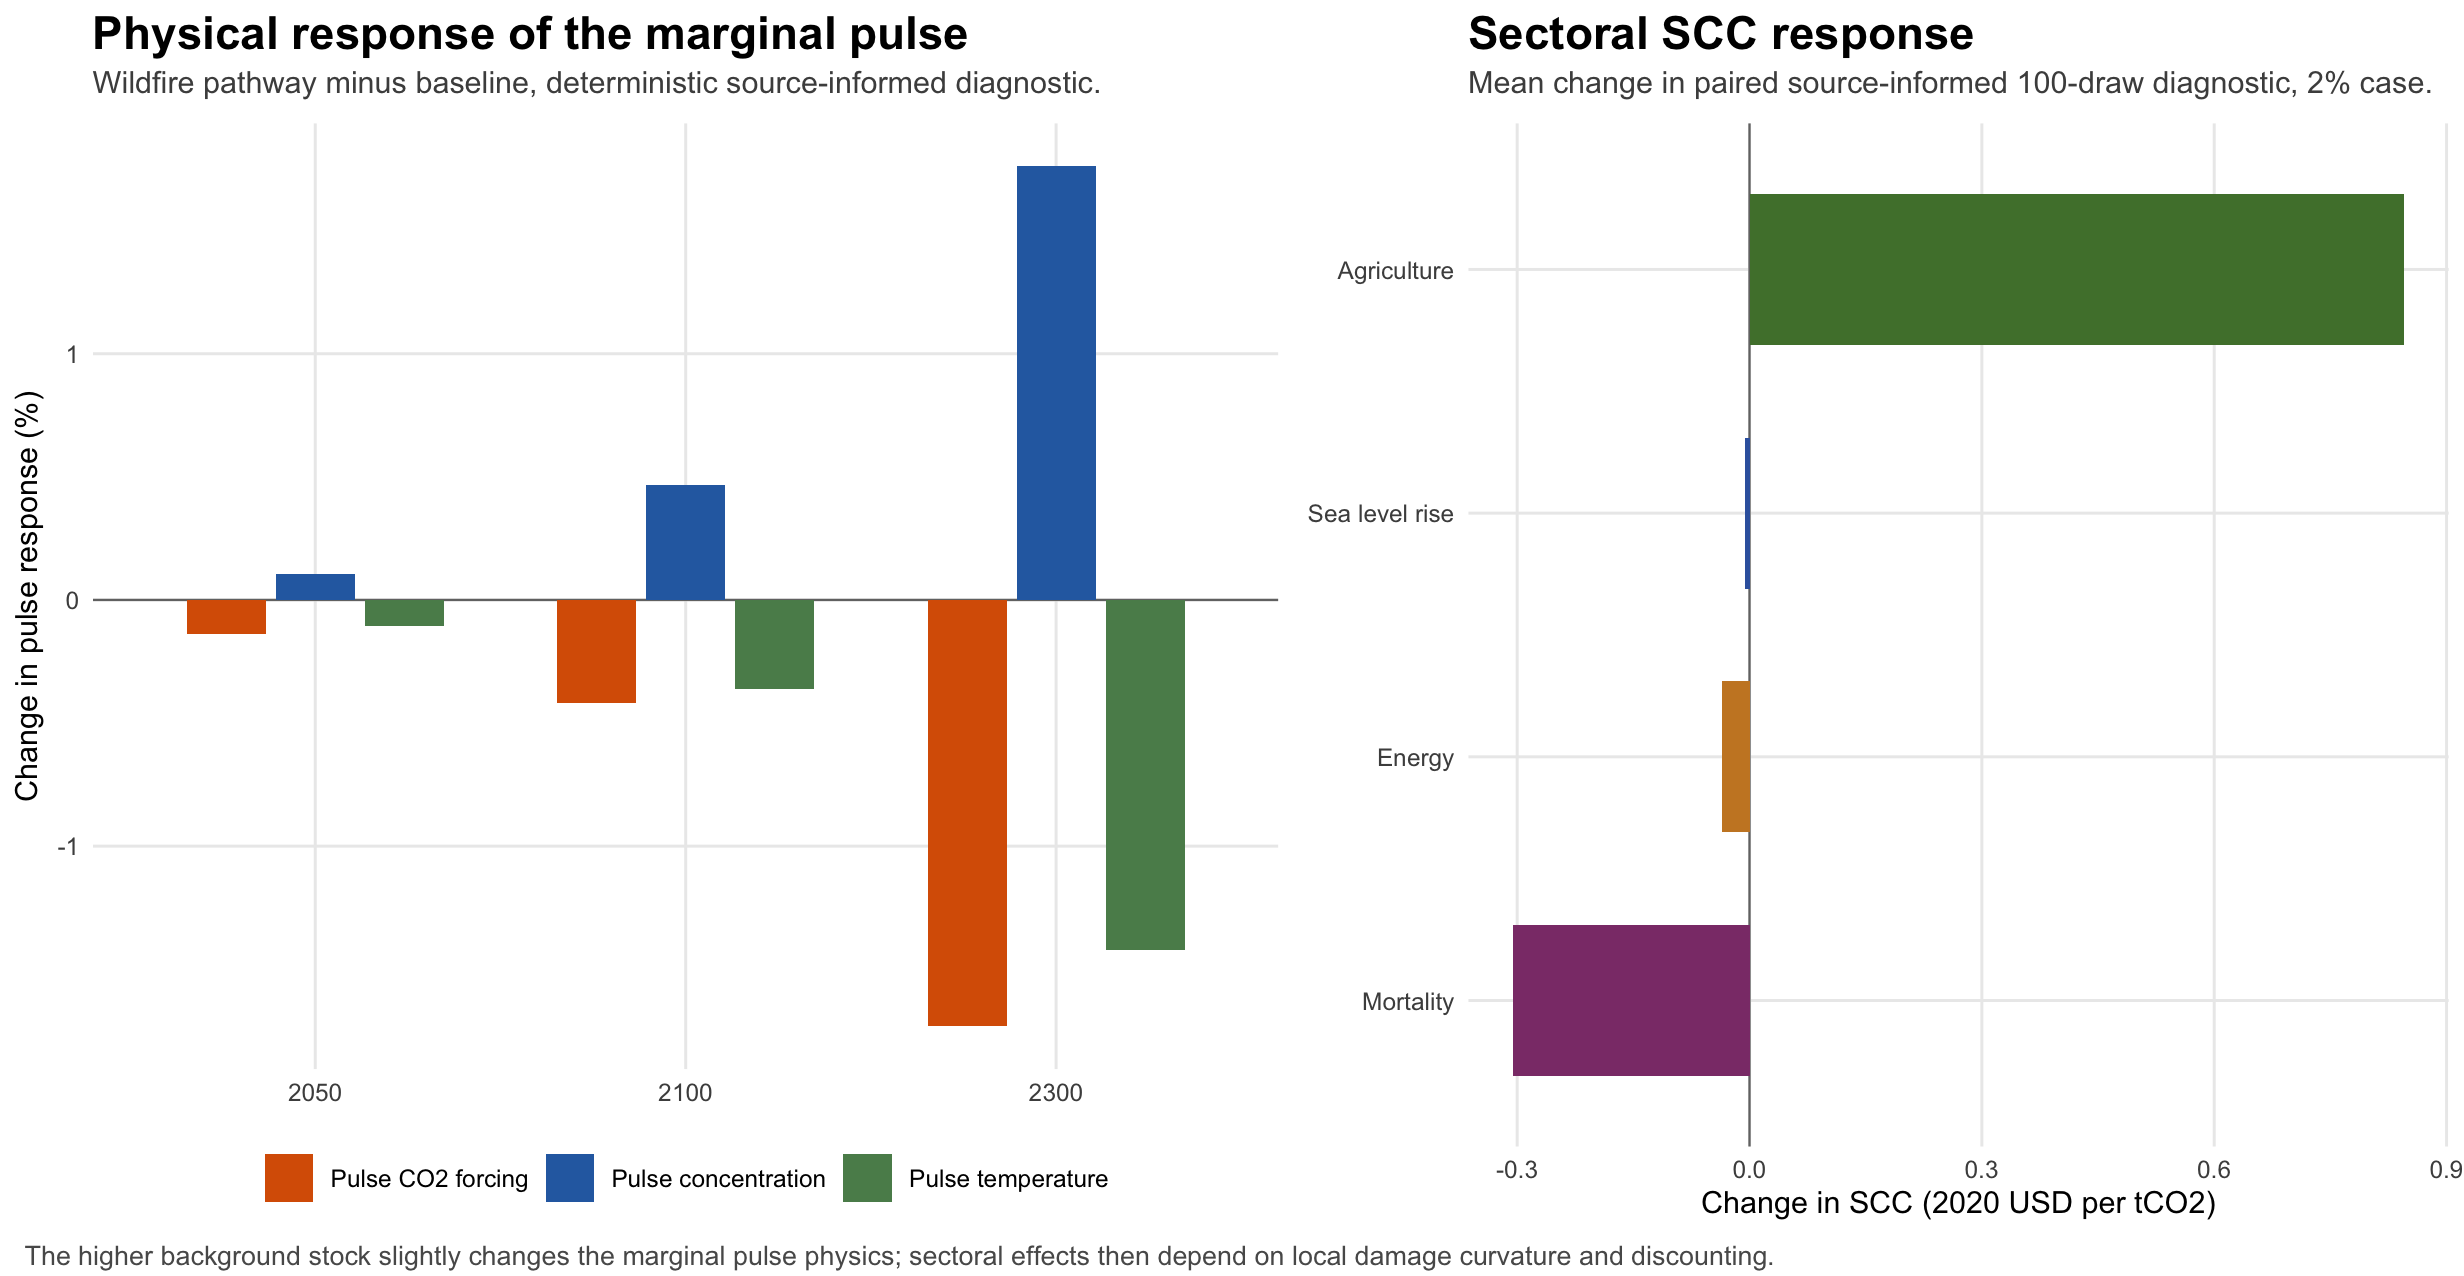
\includegraphics[keepaspectratio,alt={Mechanism decomposition. The left panel compares the marginal-pulse physical response under the source-informed wildfire pathway and baseline. The right panel decomposes the 2\% SCC response by sector in the paired source-informed diagnostic.}]{figures/png_pdf/figure_mechanism_decomposition.png}}
\caption{Mechanism decomposition. The left panel compares the
marginal-pulse physical response under the source-informed wildfire
pathway and baseline. The right panel decomposes the 2\% SCC response by
sector in the paired source-informed diagnostic.}
\end{figure}

\subsection{Discussion}\label{discussion}

The central result is an accounting result as much as a numerical
result. GIVE does not internally generate a climate-driven
wildfire-carbon feedback, so adding such a feedback is structurally
justified. But the released aggregate emissions pathway cannot identify
how much wildfire, biomass-burning, AFOLU or natural-stock carbon was
already included in the baseline. The defensible central estimate is
therefore a residual net-persistent feedback, not a gross fire-emissions
addition.

This distinction reconciles two intuitions that otherwise seem
inconsistent. Large fires can emit carbon on the scale of major national
fossil-fuel emitters, and added fire CO2 can raise concentrations,
temperature and total damages. Yet the SCC is a marginal measure. If the
same fire path is added to both the baseline and pulse worlds, the SCC
changes only through nonlinear state dependence. If the marginal tonne
itself increases fire CO2 through warming, the SCC changes through a
causal feedback, but the effect depends on how much gross fire carbon is
persistent and missing from the baseline.

The stress cases show that the mechanism can be large. When high
forest-fire projections are treated as persistent and entirely absent
from the baseline, the SCC rises substantially. Those results should not
be read as central estimates. They are upper-bound diagnostics that
reveal sensitivity to a potentially important omitted feedback. The
residual cases are more cautious because they admit uncertainty over
regrowth, land-carbon accounting and baseline embedding. The stronger
paper is therefore not a claim that gross wildfire emissions should be
added to SCC models. It is a claim that SCC models need explicit
fire-carbon accounting so analysts can distinguish gross emissions, net
atmospheric additions and baseline overlap.

The analysis also clarifies how this work relates to wildfire smoke
mortality. Qiu et al.~(2026) value the mortality benefits of reduced
smoke exposure under climate mitigation. Our extension values a
carbon-cycle feedback in which additional fire CO2 causes further
warming and damages. These channels are complementary. A complete
wildfire SCC would combine them only after specifying a common
climate-fire response model so that smoke damages, fire CO2, methane,
aerosols and ecosystem carbon are not double counted.

Several limitations are first-order. The feedback is global and reduced
form rather than spatially resolved. The persistence and missing-share
parameters are bounded but not empirically identified because the
released baseline does not expose the needed carbon-accounting
components. The model omits non-CO2 fire forcers, smoke mortality,
albedo, suppression, land management and vegetation transitions. The
current Monte Carlo numbers are 100-draw validation results; a
submission-ready production run should use a larger paired ensemble and,
ideally, a factorial uncertainty design. Finally, the SCC remains a
marginal welfare metric; it should not be used as a substitute for
reporting total damages or physical carbon-cycle risk.

The policy implication is not that SCC estimates should simply add
wildfire emissions. It is that SCC models should represent fire-carbon
accounting explicitly. Future projections should identify gross fire
emissions, net ecosystem carbon change, atmospheric persistence and the
overlap with AFOLU and natural-stock emissions baselines. Without that
accounting, analysts face a false choice between ignoring a potentially
important climate feedback and double counting carbon already embedded
in aggregate pathways.

\subsection{Methods}\label{methods}

\subsubsection{Model and pathway audit}\label{model-and-pathway-audit}

We used the Rennert et al.~replication archive and the archived GIVE
Julia environment. The audit traced how CO2 emissions enter the model,
whether wildfire or biomass burning appears as a separate pathway, and
whether the SCC pulse can alter future emissions. GIVE uses aggregate
emissions scenarios and does not contain an endogenous socioeconomic
module. Population, GDP and emissions are sampled from exogenous
pathways. In Kaya terms, emissions are not recomputed dynamically from
population, income, energy intensity and carbon intensity after climate
or damages are realized.

The RFF-SP data used by GIVE provide global CO2 emissions as an
aggregate carbon-mass pathway. The released input does not decompose CO2
into fossil, industrial-process, AFOLU, wildfire, biomass-burning,
natural-stock or negative-emissions components. For non-RFF fallback
scenarios, GIVE uses aggregate AR6 fossil CO2 and other CO2 categories.
The released model therefore cannot determine whether a specific
projected wildfire-carbon feedback is already included. Implementation
details, repository paths and reproducibility instructions are provided
in the Supplement and in the public extension repository.

\subsubsection{Wildfire-carbon feedback}\label{wildfire-carbon-feedback}

The extension adds wildfire CO2 before the CO2 pathway enters the carbon
cycle. For year t after 2020, added fire emissions are

\begin{Shaded}
\begin{Highlighting}[]
\NormalTok{E\_fire,t = E\_ref * beta * max(T[t{-}1] {-} T[2020], 0) * phi\_net * phi\_missing .}
\end{Highlighting}
\end{Shaded}

Here E\_ref is reference gross global fire carbon, beta is the
fractional gross fire-emissions response per degree C, phi\_net is the
net-persistence fraction and phi\_missing is the not-already-embedded
fraction. Lagged temperature avoids a same-year algebraic loop and
allows the marginal pulse to induce additional fire CO2 through marginal
warming. The model uses GtC internally; CO2-mass values are converted
using 1 GtC = 44/12 GtCO2.

Residual-medium samples beta from a triangular distribution with
low/mode/high values 0.07/0.10/0.15 per degree C, phi\_net from
0.05/0.10/0.20 and phi\_missing from 0.25/0.50/0.75. Residual-high
samples beta from 0.25/0.50/0.75, phi\_net from 0.15/0.30/0.50 and
phi\_missing from 0.50/0.75/1.00. The beta ranges are exploratory
literature-bounded values informed by global fire-emissions inventories,
projected fire-emissions studies and RESFire-style climate-fire feedback
work. The phi\_net ranges express the gross-to-net persistence problem
rather than a formal global posterior. The phi\_missing ranges are
accounting bounds: they cannot be identified from the released aggregate
RFF-SP CO2 pathway. RESFire half-gross and gross stress cases calibrate
beta to high forest-fire projection magnitudes and set phi\_net and
phi\_missing to one.

\subsubsection{Monte Carlo and
diagnostics}\label{monte-carlo-and-diagnostics}

Monte Carlo experiments are paired. The same RFF-SP and FaIR draw IDs,
and the same non-fire uncertainty streams, are used across baseline and
wildfire scenarios. This design makes scenario differences less noisy
than independent sampling. The validation run uses 100 paired draws. For
each scenario, we report SCC levels and draw-level paired deltas. Delta
summaries include means, medians, 2.5th, 5th, 25th, 75th, 95th and
97.5th percentiles, plus exceedance probabilities. We also compute
diagnostic proxy regressions of paired deltas on the matched baseline
SCC draw and on the effective wildfire-feedback intensity beta times
phi\_net times phi\_missing. These diagnostics separate baseline-state
and feedback-intensity variation descriptively, but they are not a
formal Sobol or ANOVA decomposition. The production driver is configured
for larger paired ensembles across baseline, residual-medium,
residual-high, half-gross stress and gross stress scenarios.

We also use deterministic diagnostics to test model wiring. Scale checks
compare annual added fire CO2 with baseline annual aggregate CO2
emissions and compare induced atmospheric carbon with the baseline
atmospheric CO2-C stock. Mechanism checks compare concentration,
forcing, temperature, damages and sectoral marginal damages under
baseline and added-fire pathways. A common exogenous-path diagnostic is
used as a negative control: when the same wildfire path is imposed in
base and pulse worlds, SCC changes only through state nonlinearities
rather than through feedback emissions caused by the pulse.

\subsubsection{AI-assisted research
programming}\label{ai-assisted-research-programming}

A generative AI coding assistant was used as a research-programming aid.
The human author specified the research question, modeling hypotheses,
acceptance criteria and interpretation. The assistant was used to
inspect replication code, identify relevant files, search and summarize
candidate literature, draft and revise Julia, R, Python and HTML
scripts, generate preliminary figures and tables, and identify unit,
model-wiring and double-counting checks. All source selection, modeling
choices, code execution, numerical results, manuscript text and
interpretation were reviewed and approved by the human author, who takes
responsibility for the accuracy and integrity of the work. The AI system
is not listed as an author because it cannot satisfy authorship
accountability criteria. A prompt-history appendix is provided for
transparency.

\subsection{Data availability}\label{data-availability}

The original GIVE replication archive is available through the Rennert
et al.~Zenodo record and GitHub repository. RFF-SP data are loaded
through the archived replication environment. The wildfire extension
repository is available at
\url{https://github.com/jbbcsu/give-wildfire-carbon-feedback}. It
contains the cleaned fire-projection summary, wildfire-parameter
framework, 100-draw validation summaries, paired-delta tables,
manuscript figures and figure-input files used in this draft. The
current public draft uses 100-draw validation outputs; production
outputs should replace them before submission.

\subsection{Code availability}\label{code-availability}

The wildfire extension is separate from the original replication code
and is archived at
\url{https://github.com/jbbcsu/give-wildfire-carbon-feedback}. It
includes the Julia model-extension module, deterministic and Monte Carlo
drivers, diagnostic scripts, figure builders, an interactive website, a
teaching module and manuscript materials. The original Rennert et
al.~replication archive should be downloaded separately and the
extension placed inside that project as \texttt{wildfire\_extension/}
for full reproduction.

\subsection{References}\label{references}

Abatzoglou, J. T. and Williams, A. P. Impact of anthropogenic climate
change on wildfire across western US forests. Proceedings of the
National Academy of Sciences 113, 11770-11775 (2016).
https://doi.org/10.1073/pnas.1607171113

Andela, N. et al.~A human-driven decline in global burned area. Science
356, 1356-1362 (2017). https://doi.org/10.1126/science.aal4108

Bowman, D. M. J. S. et al.~Fire in the Earth system. Science 324,
481-484 (2009). https://doi.org/10.1126/science.1163886

Bressler, R. D. The mortality cost of carbon. Nature Communications 12,
4467 (2021). https://doi.org/10.1038/s41467-021-24487-w

Burke, M., Hsiang, S. M. and Miguel, E. Global non-linear effect of
temperature on economic production. Nature 527, 235-239 (2015).
https://doi.org/10.1038/nature15725

Byrne, B. et al.~Carbon emissions from the 2023 Canadian wildfires.
Nature 633, 835-839 (2024). https://doi.org/10.1038/s41586-024-07878-z

Carleton, T. A. et al.~Valuing the global mortality consequences of
climate change accounting for adaptation costs and benefits. Quarterly
Journal of Economics 137, 2037-2105 (2022).
https://doi.org/10.1093/qje/qjac020

Chen, W., Zhang, Y., Zou, Y. et al.~Climate feedback of forest fires
amplified by atmospheric chemistry. Nature Geoscience 19, 402-405
(2026). https://doi.org/10.1038/s41561-026-01926-1

Diaz, D. and Moore, F. Quantifying the economic risks of climate change.
Nature Climate Change 7, 774-782 (2017).
https://doi.org/10.1038/nclimate3411

Friedlingstein, P. et al.~Global Carbon Budget 2023. Earth System
Science Data 15, 5301-5369 (2023).
https://doi.org/10.5194/essd-15-5301-2023

Friedlingstein, P. et al.~Global Carbon Budget 2024. Earth System
Science Data 17, 965-1039 (2025).
https://doi.org/10.5194/essd-17-965-2025

Ford, B. et al.~Future fire impacts on smoke concentrations, visibility,
and health in the contiguous United States. GeoHealth 2, 229-247 (2018).
https://doi.org/10.1029/2018GH000144

Giglio, L., Randerson, J. T. and van der Werf, G. R. Analysis of daily,
monthly, and annual burned area using the fourth-generation global fire
emissions database (GFED4). Journal of Geophysical Research:
Biogeosciences 118, 317-328 (2013). https://doi.org/10.1002/jgrg.20042

Howard, P. H. and Sterner, T. Few and not so far between: a
meta-analysis of climate damage estimates. Environmental and Resource
Economics 68, 197-225 (2017). https://doi.org/10.1007/s10640-017-0166-z

Jolly, W. M. et al.~Climate-induced variations in global wildfire danger
from 1979 to 2013. Nature Communications 6, 7537 (2015).
https://doi.org/10.1038/ncomms8537

Jones, M. W., Santin, C., van der Werf, G. R. et al.~Global fire
emissions buffered by the production of pyrogenic carbon. Nature
Geoscience 12, 742-747 (2019). https://doi.org/10.1038/s41561-019-0403-x

Kopp, R. E. et al.~Probabilistic 21st and 22nd century sea-level
projections at a global network of tide-gauge sites. Earth's Future 2,
383-406 (2014). https://doi.org/10.1002/2014EF000239

Leach, N. J. et al.~FaIRv2.0.0: a generalized impulse response model for
climate uncertainty and future scenario exploration. Geoscientific Model
Development 14, 3007-3036 (2021).
https://doi.org/10.5194/gmd-14-3007-2021

Millar, R. J. et al.~Emission budgets and pathways consistent with
limiting warming to 1.5 C. Nature Geoscience 10, 741-747 (2017).
https://doi.org/10.1038/ngeo3031

Moore, F. C., Baldos, U., Hertel, T. and Diaz, D. New science of climate
change impacts on agriculture implies higher social cost of carbon.
Nature Communications 8, 1607 (2017).
https://doi.org/10.1038/s41467-017-01792-x

Moritz, M. A. et al.~Climate change and disruptions to global fire
activity. Ecosphere 3, 49 (2012). https://doi.org/10.1890/ES11-00345.1

National Academies of Sciences, Engineering, and Medicine. Valuing
Climate Damages: Updating Estimation of the Social Cost of Carbon
Dioxide. National Academies Press (2017). https://doi.org/10.17226/24651

Nature Portfolio. Artificial Intelligence (AI) editorial policy.
Springer Nature (accessed 12 June 2026).
https://www.nature.com/nature-portfolio/editorial-policies/ai

Nordhaus, W. D. Revisiting the social cost of carbon. Proceedings of the
National Academy of Sciences 114, 1518-1523 (2017).
https://doi.org/10.1073/pnas.1609244114

Pechony, O. and Shindell, D. T. Driving forces of global wildfires over
the past millennium and the forthcoming century. Proceedings of the
National Academy of Sciences 107, 19167-19170 (2010).
https://doi.org/10.1073/pnas.1003669107

Piontek, F. et al.~Integrated perspective on translating biophysical to
economic impacts of climate change. Nature Climate Change 11, 563-572
(2021). https://doi.org/10.1038/s41558-021-01065-y

Prest, B. C. et al.~The social cost of carbon: advances in long-term
probabilistic projections of population, GDP, emissions, and discount
rates. Brookings Papers on Economic Activity 2021(2), 223-305 (2022).
https://doi.org/10.1353/eca.2022.0003

Qiu, M. et al.~Valuing wildfire smoke-related mortality benefits from
climate mitigation. Proceedings of the National Academy of Sciences 123,
e2533772123 (2026). https://doi.org/10.1073/pnas.2533772123

Rennert, K. et al.~Comprehensive evidence implies a higher social cost
of CO2. Nature 610, 687-692 (2022).
https://doi.org/10.1038/s41586-022-05224-9

Ricke, K., Drouet, L., Caldeira, K. and Tavoni, M. Country-level social
cost of carbon. Nature Climate Change 8, 895-900 (2018).
https://doi.org/10.1038/s41558-018-0282-y

Rode, A. et al.~Estimating a social cost of carbon for global energy
consumption. Nature 598, 308-314 (2021).
https://doi.org/10.1038/s41586-021-03883-8

Tol, R. S. J. The social cost of carbon. Annual Review of Resource
Economics 3, 419-443 (2011).
https://doi.org/10.1146/annurev-resource-083110-120028

van der Werf, G. R. et al.~Global fire emissions estimates during
1997-2016. Earth System Science Data 9, 697-720 (2017).
https://doi.org/10.5194/essd-9-697-2017

Val Martin, M., Pierce, J. R. and Heald, C. L. Global fire emissions,
fire area burned and air quality data projected using a global earth
system model (RCP45/SSP1 and RCP8.5/SSP3). Forest Service Research Data
Archive (2018; updated 2021). https://doi.org/10.2737/RDS-2018-0021

Walker, X. J. et al.~Increasing wildfires threaten historic carbon sink
of boreal forest soils. Nature 572, 520-523 (2019).
https://doi.org/10.1038/s41586-019-1474-y

Wong, T. E. et al.~BRICK v0.2, a simple, accessible, and transparent
model framework for climate and regional sea-level projections.
Geoscientific Model Development 10, 2741-2760 (2017).
https://doi.org/10.5194/gmd-10-2741-2017

Zheng, B. et al.~Record-high CO2 emissions from boreal fires in 2021.
Science 379, 912-917 (2023). https://doi.org/10.1126/science.ade0805

Zou, Y. et al.~Development of a REgion-Specific ecosystem feedback Fire
(RESFire) model in the Community Earth System Model. Journal of Advances
in Modeling Earth Systems 11, 417-445 (2019).
https://doi.org/10.1029/2018MS001368

Zou, Y. et al.~Using CESM-RESFire to understand climate-fire-ecosystem
interactions and the implications for decadal climate variability.
Atmospheric Chemistry and Physics 20, 995-1020 (2020).
https://doi.org/10.5194/acp-20-995-2020
